\section{Control File}
\subsection{Overview of Control File}
These listed model features are denoted in the control file in the following order:
	\begin{enumerate}
		\item Number of growth patterns and platoons
		\item Design matrix for assignment of recruitment to area/settle\_event/growth pattern
		\item Design matrix for movement between areas
		\item Definition of time blocks that can be used for time-varying parameters
		\item Controls far all time-varying parameters
		\\
		\item Specification for growth and fecundity
		\item Natural mortality and growth parameters for each sex x growth pattern
		\item Maturity, fecundity and weight-length for each sex
		\item Recruitment distribution parameters for each area, settle\_event, growth pattern
		\item Cohort growth deviation
		\item Movement between areas
		\item Catch Multiplier
		\item Fraction female
		\item Setup for any MG parameters are time-varying
		\item Seasonal effects on biology parameters
		\\
		\item Spawner-recruitment parameters
		\item Setup for any SR parameters are time-varying
		\item Recruitment deviations
		\\
		\item F ballpark value in specified year
		\item Method for calculating fishing mortality (F)
		\item Initial equilibrium F for each fleet
		\\
		\item Catchability (Q) setup for each fleet and survey
		\item Catchability parameters
		\item Setup for any Q parameters are time-varying
		\\
		\item Length selectivity, retention, discard mortality setup for each fleet and survey
		\item Age selectivity setup for each fleet and survey
		\item Parameters for length selectivity, retention, discard mortality for each fleet and survey
		\item Parameters for age selectivity, retention, discard mortality for each fleet and survey
		\item Setup for any selectivity parameters are time-varying
		\\
		\item Tag-recapture parameters
		\\
		\item Variance adjustments
		\item Lambdas for likelihood components
	\end{enumerate}
The order in which they appear in the control file has grown over time rather opportunistically, so it may not appear particularly logical at this time, especially various aspects of recruitment distribution and growth.  When the same information is entered via the GUI, it is organized more logically and then written in this form to the text control file.


\subsection{Parameter Line Elements}
The primary role of the SS control file is to define the parameters to be used by the model.  The general syntax of the 14 elements of a long parameter line is described here.  The first seven elements of a parameter line are used for time-varying parameters that cannot themselves be time-varying and will be referred to as a short parameter line.  Three types of time-varying properties can be applied to a base parameter:  blocks or trend, environmental linkage, and random deviation.  Each parameter line contains:

\hypertarget{Priors}{} \hypertarget{paraOrder}{}
\begin{center}
	\begin{tabular}{p{2cm} p{3cm} p{10cm}}
		\hline
		Column & Element & Description \Tstrut\Bstrut\\
		\hline
		1 & LO & Minimum value for the parameter\Tstrut\\
		2 & HI & Maximum value for the parameter\Tstrut\\
		3 \Tstrut & INIT & Initial value for the parameter.  If the ss.par file is read, it overwrites these INIT values.\\
		4 \Tstrut & PRIOR & Expected value for the parameter.  This value is ignored if the prior type is 0 (no prior) or 1 (symmetric beta).\\
		5 \Tstrut & PRIOR STDEV & Standard deviation for the prior, used to calculate likelihood of the current parameter value. This value is ignored if prior type is 0.\\
		6 \Tstrut & \hyperlink{PriorDescrip}{PRIOR TYPE}  & 0 = none, \\
		& & 1 = symmetric beta, \\
		& & 2 = full beta, \\
		& & 3 = lognormal without bias adjustment, \\
		%& & ($Pr_{\text{like}} = 0.5((log(P_{\text{val}}) -Pr)/Pr_{\text{sd}})^2$), \\
		& & 4 = lognormal with bias adjustment, \\
		%8 8 ($Pr_{\text{like}} = 0.5((log(P_{\text{val}}) -Pr+0.5*Pr_{\text{sd}}^2)/Pr_{\text{sd}})^2$), \\
		& & 5 = gamma, \\
		& & 6 = normal. \\
		7 \Tstrut & PHASE & Phase in which parameter begins to be estimated.  A negative value causes the parameter to retain its INIT value (or value read from the ss.par file).\Bstrut\\
		\hline
	\end{tabular}
\end{center}

Note that relative to SS v.3.24,  the order of Prior StDev and Prior Type have been switched and the Prior Type options have been renumbered.

Short parameter lines have only the above 7 elements.  The full parameter line syntax for the mortality-growth, spawn-recruitment, selectivity, and Q sections provides additional controls to give the parameter time-varying properties.  These are listed briefly below and described in more detail in the section time varying parameter options found in the \hyperlink{TVpara}{Time-Varying parameters} section.

\begin{center}
	\begin{tabular}{p{2cm} p{3cm} p{10cm}}
		\hline
		Column & Element & Description \Tstrut\Bstrut\\
		\hline
		8  & Env Var \& Link & Create a linkage to an input environmental time-series\Tstrut\Bstrut\\
		9  \Tstrut & Dev Link & Invokes use of the deviation vector in the linkage function \\
		10 \Tstrut & Dev min yr & Beginning year for the deviation vector \\
		11 \Tstrut & Dev max yr & Ending year for the deviation vector\\
		12 \Tstrut & Dev Phase & Phase for estimation for elements in the deviation vector \\
		13 \Tstrut & Block & Specify time block or trend to be applied \\
		14 \Bstrut & Block Function & Function form for the block offset\\
		\hline
	\end{tabular}
\end{center}

\subsection{Terminology}
Where the term “COND” appears in the value column of this documentation (it does not actually appear in the control file), it indicates that the following section is omitted except under certain conditions, or that the factors included in the following section depend upon certain conditions.
In most cases, the description in the Definition column is the same as the label output to the control.ss\textunderscore new file.

\subsection{Beginning of Control File Inputs}
\begin{center}
	\begin{longtable}{p{0.5cm} p{2cm} p{12cm}}
		\hline
		\multicolumn{2}{l}{Typical Value} & Description and Options\Tstrut\Bstrut\\
		\hline
		\endfirsthead

		\hline
		\multicolumn{2}{l}{Typical Value} & Description and Options\Tstrut\Bstrut\\
		\hline
		\endhead

		\hline
		\endfoot

		\endlastfoot

		\multicolumn{2}{l}{\#C comment }\Tstrut & Comments beginning with \#C at the top of the file will be retained and included in output. \Bstrut\\
		\hline

		0 & & 0 = do not read the wtatage.ss file, \Tstrut\\
		  & & 1 = read the wtatage.ss file, also read and use the growth parameters, \\
		  & & 2 = Future option to read the wtatage.ss file, then omit reading and using growth parameters and all length-based data.\Bstrut\\

		%\hline
		\pagebreak
		2 & & N growth patterns (GP)\Tstrut\\
		& & These are collections of fish with unique biological characteristics (growth, M, wt-len, reproduction.)  The GP x Sex x Settlement Events constitute unique morphs that are tracked in SS.  They are assigned these characteristics at birth and retain them throughout their lifetime.  At recruitment, morph members are distributed across areas (if any) and they retain their biological characteristics even if they move to another area in which a different cohort with different biological characteristics might predominate.  For example, one could assign a fast-growing morph to recruit predominately in a southern areas and a slow-growing morph to a northern area.  The natural mortality and growth parameters are specified for each growth pattern in the MG parameters section in the order of females growth pattern 1 to growth pattern N followed by males growth pattern 1 to growth pattern N.\Bstrut\\

		\hline
		3 & & Number of platoons within a morph.\Tstrut\\
		& & This allows exploration of size-dependent survivorship. A value of 1 will not create additional platoons.  Odd-numbered values of 3 - 5 will break the overall morph into that number of platoons.  More platoons slows model execution, so values above 5 not advised.  The fraction of each morph assigned to each platoon is custom-input or designated to be a normal approximation.  When multiple platoons are designated, an additional input is the ratio of between platoon to within platoon variability in size-at-age.  This is used to partition the total growth variability.  For the platoons, their size-at-age is calculated as a factor (determined from the between-within variability calculation) times the size-at-age of the central morph which is determined from the growth parameters for that Growth Pattern x Sex. \Bstrut\\

		\multicolumn{2}{l}{COND > 1}& \multicolumn{1}{l}{\parbox{12cm}{Following 2 lines are conditional on N platoons > 1}} \Tstrut\Bstrut\\

		& 0.7 & Platoon between/within stdev ratio. Ratio of the amount of variability in length-at-age between platoons to within platoons.\Bstrut\\
		%\hline

		& 0.2 0.6 0.2 & Distribution among platoons. Enter custom vector or enter -1 to first value of vector to get a normal approximation: (0.15, 0.70, 0.15) for 3 platoons, (0.031, 0.237, 0.464, 0.237, 0.031) for 5 platoons.\Bstrut\\
		\hline
	\end{longtable}
\end{center}

\subsubsection{Empirical Weight-at-Age}
With version 3.04, SS added the capability to read empirical body weight at age for the population and each fleet, in lieu of generating these weights internally from the growth parameters, weight-at-length, and size-selectivity.  The values are read from a separate file named, wtatage.ss.  This file is only required to exist if this option is selected.  See the section on \hyperlink{WAA}{weight-at-age} for additional information on file formatting for empirical weight-at-age.


\subsubsection{Recruitment Timing and Distribution}
In older versions of SS one value of spawning biomass was calculated annually at the beginning of one specified spawning season and this spawning biomass produces one annual total recruitment value and this annual recruitment was distributed among seasons, areas, and growth types according to other model parameters.\\ 

In SS v.3.30, more control of the seasonal timing is provided and there now is an explicit time delta between spawning and recruitment. Spawning still occurs just once per year, but its timing can be at any specified time, not just the beginning of a season.  Recruitment of the progeny from an annual spawning enter the population in one or more settlement events.  

\begin{center}
	\begin{tabular}{p{3cm} p{2cm} p{2cm} p{7cm}}
		\multicolumn{4}{l}{Example set-up where there are multiple settlement events:}\\
		\hline
		3 & \multicolumn{3}{l}{Number of recruitment settlement events}\Tstrut\\
		0 & \multicolumn{3}{l}{Unused option}\Bstrut\\
		\hline
		Growth Pattern & Month & Area & Age (for each settlement assignment)\Tstrut\Bstrut\\
		\hline
		1 & 11.0 & 1 & 0 \Tstrut\\
		1 & 12.0 & 1 & 0 \\
		1 & 1.0  & 1 & 1 \Bstrut\\
		\hline
	\end{tabular}		
\end{center}

%\begin{description}
%	\item[Recruitment Timing and Settlement]\
\myparagraph{Recruitment Timing and Settlement}
Details regarding recruitment timing and settlement:
	\begin{itemize}
		\item Recruitment happens in specified settlement events (growth pattern, Month, Area);
		\item Number of unique settlement timings calculated at runtime;
		\item Now there is explicit elapsed time between spawning and recruitment;
		\item Growth and natural mortality of the platoon begins at time of settlement, which is its real age 0.0 for growth; but pre-settlement fish exist from the beginning of the season of settlement, so can be caught if selected;
		\item Age at recruitment now user-controlled (should be 0 if in year of spawning)
		\item All fish become integer age 1 (for age determination) on their first January 1st;
		\item Recruitment can occur >12 months after spawning		
	\end{itemize}
%\end{description}

The distribution of recruitment among these settlement events is controlled by recruitment apportionment parameters. There must be a parameter line for each GP, then for each area, then for each settlement.  All of these are required, but only those GP x area x settlements designated to receive recruits in the recruitment design matrix will have the parameter used in the recruitment distribution calculation.  For the recruitment apportionment, the parameter values are the ln(apportionment weight).  The sum of all apportionment weights is calculated for each pattern x area x settlements that have been designated to receive recruits in the recruitment design matrix.  Then the apportionment weights are scaled to sum to 1.0 so that the total recruitment from the spawning event is distributed among the cells designated to receive recruitment. These distribution parameters can be time-varying, so the fraction of the recruits that occur in a particular GP, area, or settlement can change from year to year. 

%\begin{description}
%	\item[Recruitment Distribution Parameters]\
\myparagraph{Recruitment Distribution and Parameters}
	\begin{itemize}
		\item SS processes the parameter values according to the following equation:
		\begin{equation}
		\text{apportionment}_i = \frac{e^{p_i}}{\sum_{j=1}^{N}e^{p_i}}
		\end{equation}
		\item Set the value for one of these parameters to 0.0 and not estimate it so that other parameters will be estimated relative to its fixed value.
		\item Give the estimated parameters a min-max of something like -5 and 5, so they have a good range relative to the base parameter.
		\item In order to get a different distribution of recruitments in different years, you will need to make at least one of the recruitment distribution parameters time-varying.
		\item In a seasonal model, all cohorts graduate to the age of 1 when they first reach January 1, even if the seasonal structure of the model has them being born in the late fall.  In general, this means that SS operates under the assumption that all age data have been adjusted so that fish are age 0 at the time of spawning and all fish graduate to the next age on Jan 1.  This can be problematic if the ageing structures deposit a ring at another time of year.  Consequently, you may need to add or subtract a year to some of your age data to make it conform to the SS structure, or you may need to define the SS calendar year to start at the beginning of the season at which ring deposition occurs.  Talk with your ageing lab about their criteria for seasonal ring deposition!
		\item Seasonal recruitment is coded to work smoothly with growth.  If the recruitment occurring in each season is assigned the same growth pattern, then each seasonal cohort’s growth trajectory is simply shifted along the age/time axis.  At the end of the year, the early born cohorts will be larger, but all are growing with the same growth parameters so all will converge in size as they approach their common Lmax.
		\item At the time of settlement, fish are assigned a size equal to the lower edge of the first population size bin and they grow linearly until they reach the age A1.  SS generates a warning if the first population length bin is greater than 10 cm as this seems an unreasonably large value for a larval fish.  A1 is in terms of real age elapsed since birth.  All fish advance to the next integer age on Jan 1, regardless of birth season.  For example, consider a 2 season model with some recruitment in each season and with each season’s recruits coming from the same GP.  At the end of the first year, the early born fish will be larger but both of the seasonal cohorts will advance to an integer age of 1 on Jan 1 of the next year.  The full growth curve is still calculated below A1, but the size-at-age used by SS is the linear replacement.  Because the linear growth trajectory can never go negative, there is no need for the additive constant to the standard deviation (necessary for the growth model used in SS2 V1.x), but the option to add a constant has been retained in the model.
	\end{itemize}
%\end{description}
	
	
\begin{longtable}{p{0.5cm} p{2cm} p{12cm}}
	\hline
	\multicolumn{2}{l}{Typical Value} & Description and Options\Tstrut\Bstrut\\
	\hline
	\endfirsthead

	\hline
	\multicolumn{2}{l}{Typical Value} & Description and Options\Tstrut\Bstrut\\
	\hline
	\endhead

	\hline
	\endfoot

	\endlastfoot

	%\hline
	%\multicolumn{2}{l}{Typical Value} & Description \Tstrut\Bstrut\\
	%\hline		
	1 \Tstrut & & Recruitment distribution method. This section controls which combinations of Growth Pattern x Area x Settlement will get a portion of the total recruitment coming from each spawning.  Options: \\
	  & & 1 = use the SS v.3.24 or earlier setup, \\
	  & & 2 = main effects for GP, settle timing, and area, \\
	  & & 3 = each settle entity, \\
	  & & 4=no parameters (only if Growth Pattern x Settlement x Area = 1). \Bstrut\\

	\hline
	1 & & Spawner-Recruitment, options: \Tstrut\\
	  & & 1 = global, \\
	  & & 2 = by area (by area is not yet implemented; there is a conceptual challenge to doing the equilibrium calculation when there is fishing).\Bstrut\\

	\hline
	1 \Tstrut & & Number of recruitment settlement assignments.  Must be at least 1 even if only 1 settlement and 1 area because the timing of that settlement must be specified.\Bstrut\\

	\hline
	0 \Tstrut & & Year x Area x Settlement Event Interaction Requested (only for recruitment distribution method = 1). \Bstrut\\

	\hline
	\multicolumn{2}{l}{1 5.5 1 0} \Tstrut & Recruitment assignment to growth pattern, month, area, and age (for each settlement event).  Here settlement is set to mid-May (month 5.5). Note:  Normally the calendar age at settlement is 0 if settlement happens between the time of spawning and the end of that year, and at age 1 if settlement is in the year after spawning.  In SS v.3.24, settlement always happened at age 0 even if in following year.  That is illogical, but this age option allows replication of SS v.3.24 for testing purposes.
	\Bstrut\\
	\hline
\end{longtable}


\subsubsection{Movement}
Here we define movement among the areas.  This is a box transfer with no explicit adjacency of areas, so fish can move from any area to any other area in each time step.  Future Need:  augment the capability further to allow sex-specific movement, and also to allow some sort of mirroring so that sexes and growth patterns can share the same movement parameters if desired.

\begin{longtable}{p{0.5cm} p{2cm} p{12cm}}
	\hline
	\multicolumn{2}{l}{Typical Value} & Description and Options\Tstrut\Bstrut\\
	\hline
	\endfirsthead

	\hline
	\multicolumn{2}{l}{Typical Value} & Description and Options\Tstrut\Bstrut\\
	\hline
	\endhead

	\hline
	\endfoot

	\endlastfoot
	
	\multicolumn{3}{l}{COND:  only if areas > 1}\Tstrut\\ 
	& 4   & Enter Number of movement definitions.\Tstrut\\		
	\Tstrut & 1.0  & First age that moves. This value is a real number, not an integer, to allow for an in-year start to movement in a multi-season model.  It is the real age at the beginning of a season, even though movement does not occur until the end of the season. For example, in a  setup with two 6-month seasons a value of 0.5 will cause the age 0 fish to not move when they complete their first 6 month season of life, and then to move at the end of their second season because they start movement capability when they reach the age of 0.5 years (6 months). \\
	\Tstrut & 1 1 1 2 4 10 & \multicolumn{1}{l}{\multirow{5}{6cm}{\parbox{12cm}{The four requested movement definitions appear here.  Each definition specifies: season, morph, source area, destination age1, age2. The rate of movement will be controlled by the movement parameters later.  Here the age1 and age2 controls specify the range over which the movement parameters are interpolated with movement constant below age1 and above age2.}}}\\
	& 1 1 2 1 4 10 &  \Tstrut\\
	& 1 2 1 2 4 10 &  \\
	& 1 2 2 1 4 10 &  \Bstrut\\
	\\ 
	\hline
	\end{longtable}

Two parameters will be entered later for each growth pattern, area pair and season.   
\begin{itemize}
	\item movement is constant at P1 below the specified minage for movement change, constant at P2 above maxage for movement change, and linearly interpolated for intermediate ages;
	\item For each source area the implicit movement parameter value is 0.0, but this default value is replaced if the stay movement is selected to have an explicit pair of parameter (e.g. specify movement rate for area 1 to area 1).
	\item the parameter is exponentiated so that a movement parameter value of 0 becomes 1.0;
	\item for each source area, all movement rates are then summed and divided by this sum so that 100\% of the fish are accounted for in the movement calculations;
	\begin{equation}
	\text{rate}_i = \frac{e^{p_i}}{\sum_{j=1}^{N}e^{p_i}}
	\end{equation}
	\item at least one movement parameter must be fixed so that all other movement parameters are estimated relative to it.  This is achieved naturally by not specifying the stay rate parameter so it has a fixed value of 0.0;
	\item the resultant movement rates are multiplied by season duration in a seasonal model;	
\end{itemize}


\subsubsection{Time Blocks}
	
\begin{longtable}{p{0.5cm} p{2cm} p{12cm}}
		\hline
		\multicolumn{2}{l}{Typical Value} & Description and Options\Tstrut\Bstrut\\
		\hline
		\endfirsthead
		
		3 \Tstrut & & \multirow{1}{4cm}[-0.1cm]{\parbox{12cm}{Number of block patterns. These patterns can be referred to in the parameter sections to create a separate parameter value for each block.}}\\
		\\
		\\

		\hline
		\multicolumn{2}{l}{COND > 0:} \Tstrut & \multicolumn{1}{l}{Following inputs are omitted if N Block patterns equals 0.}\\
		& \multirow{1}{2cm}[-0.1cm]{ 3 2 1 } & Blocks per pattern\\ \\

		& \multirow{1}{2cm}[-0.1cm]{1975 1985 1986 1990 1995 2001} & \multirow{3}{12cm}[-0.1cm]{Beginning and ending years for blocks in design 1; years not assigned to a block period retain the baseline value for a parameter that uses this pattern.}\\
		\\
		\\
		\\
		& \multirow{1}{2cm}[-0.1cm]{1987 1990 1995 2001} & \multirow{1}{12cm}[-0.1cm]{Beginning and ending years for blocks in design 2.}\\
		\\
		\\
		& \multirow{1}{2cm}[-0.1cm]{1999 2002} & \multirow{1}{12cm}[-0.10cm]{Beginning and ending years for blocks in design 3.}\Bstrut\\
		\hline
\end{longtable}

When using time blocks, it is important to consider which parameters will affect which years of the time series.  There are three main situations:
\begin{enumerate}
	\item Offset approach: One or more time blocks are created and cover all or a subset of the years.  Each block gets a parameter that is used as an offset from the base parameter.  In this situation you typically will allow SS to estimate the base parameter and each of the offset parameters.  In years not covered by blocks, the base parameter alone is used.  However, if blocks cover all the years, then the value of the block parameter is completely correlated with the mean of the block offsets, so model convergence and variance estimation could be affected.  The recommended approach when using offsets is to not have all the years be covered by blocks when doing offsets, or to fix the base parameter value at a reasonable level when doing offsets for all years.	
	\item Replacement approach-Option A: Here time blocks are created which cover a subset of the years.  The base parameter is used in the non-block years and the value of that base parameter is replaced by the block parameter in each respective block.  In this situation, you typically allow SS to estimate the base parameter and each of the block parameters.	
	\item Replacement-Option B: Here replacement time blocks are created for all the years.  In this case the base parameter is simply a placeholder that is always replaced by a block parameter.   In this situation, do not allow SS to estimate the base parameter and only estimate the corresponding block replacement parameters, otherwise, the search algorithm will be attempting to estimate parameters that do not contribute to the log-likelihood, so model convergence and variance estimation could be effected.  Note however, that the minimum and maximum for the base parameter are used as checks on the minimum and maximum of the blocks.
\end{enumerate}

Regardless of the block set-up approach, special consideration should be given regarding which parameter values are should be applied during forecast years.  The model will default to use all base parameter values during the forecast period.  However, there are controls in the forecast file which allow the user to specify specific parameter years to be applied during the forecast period for selectivity, relative F, and recruitment.  

%For some reason the doc crashes without this pagebreak here...
%\pagebreak
\subsubsection{Time-varying Parameter Controls}
In SS v.3.30, several changes are introduced to the implementation of time-varying parameters:

\begin{itemize}
  \item	Time-varying parameters for biology, spawner-recruitment, catchability, and selectivity are implemented using the same approach and share code.
  \item The block feature that allowed input of one block parameter line and replication of that line by SS as often as needed has been replaced.  Now there is a complete time-varying parameter auto-generation capability.
  \item The logistic bound constraint is no longer implemented due to the challenges it created to interpreting parameter values.  Instead, the auto-generate feature now creates bounds on time-varying parameters for blocks such that the combination of a bounded  value of the time-varying parameter and the base parameter will not violate the base parameter bounds.
  \item For more information on the implementation of time-varying parameters, see the \hyperlink{TVpara}{Using Time-varying Parameters} section
\end{itemize}	
	
\begin{longtable}{p{0.5cm} p{2cm} p{12cm}}
	\hline
	\multicolumn{2}{l}{Typical Value} & Description and Options\Tstrut\Bstrut\\
	\hline
	\endfirsthead

	\hline
	\multicolumn{2}{l}{Typical Value} & Description and Options\Tstrut\Bstrut\\
	\hline
	\endhead

	\hline
	\endfoot

	\endlastfoot

	1 & & Environmental/Block/Deviation adjust method for all time-vary parameters. \Tstrut\\
	  & & 1 = warning relative to base parameter bounds, \\
	  & & 3 = no bound check). Note: logistic bound check form previous SS versions (e.g., SS v.3.24) is no longer an option.\Bstrut\\

	\multicolumn{2}{l}{0 0 0 0 0} & Five values control auto-generation for: 1-biology, 2-spawnrecr, 3-catchability, 4-tag (future), 5-selectivity.\\
	&			& The accepted values are:\Tstrut\\
	&           & 0 = auto-generate all time-varying parameters,\\
	& 			& 1 = read each time-varying parameter line,\\
	&			& 2 = read each line and auto-generation if read value for parameter min = -12345. \Bstrut\\
	\hline
\end{longtable}


\subsection{Biology}
\subsubsection{Natural Mortality}
Natural mortality (M) has some options that are referenced to integer age, and some to real age since settlement.  So, if M varies by age, M will change by season and cohorts born  early in the year will have different M than late born cohorts.

Lorenzen natural mortality is based on the concept that natural mortality varies over the life cycle of a fish, which is driven by physiological and ecological processes.  So, natural mortality is scaled by the length of the fish.

\begin{longtable}{p{0.5cm} p{2cm} p{12.75cm}}
	\hline	
	\multicolumn{2}{l}{Typical Value} & Description and Options\Tstrut\Bstrut\\
	\hline
	\endfirsthead

	\hline
	\multicolumn{2}{l}{Typical Value} & Description and Options\Tstrut\Bstrut\\
	\hline
	\endhead
	\hline

	\endfoot
	
	\endlastfoot

	1 & & Natural Mortality Options:\Tstrut\\
	  & & 0 = A single parameter,\\
	  & & 1 = N breakpoints,\\
	  & & 2 = Lorenzen, \\
	  & & 3 = Read age specific M and do not do seasonal interpolation.\\
	  & & 4 = Read age specific and do seasonal interpolation, if appropriate.\Bstrut\\
	\hline

	\multicolumn{2}{l}{COND = 0} & No additional natural mortality controls. \Tstrut\Bstrut\\
	\hline

	\multicolumn{2}{l}{COND = 1} & \Tstrut\Bstrut\\
	& 4 & Number of breakpoints.  Then read a vector of ages for these breakpoints. Later, per sex x GP, read N parameters for the natural mortality at each breakpoint.\\

	\multicolumn{2}{r}{2.5 4.5 9.0 15.0} & Vector of age breakpoints. \Bstrut\\
	\hline
	
	\multicolumn{2}{l}{COND = 2} & \Tstrut\\
	& 4 \Tstrut & Reference age for Lorenzen Natural Mortality: read one additional integer value that is the reference age. Later read one parameter for each sex x growth pattern that will be the M at the reference age.  Other ages will have an M scaled to its body size-at-age.  However, if platoons are used, all will have the same M as their growth pattern.  Lorenzen M calculation will be updated if the starting year growth parameters are active, but if growth parameters vary during the time-series, the M is not further updated.  So be careful in using Lorenzen when there is time-varying growth.\\
	\hline
	
	\multicolumn{2}{l}{COND = 3 or 4} \Tstrut & Do not read any natural mortality parameters.  With option 2, these M values are held fixed for the integer age (no seasonality or birth season considerations). With option 4, there is seasonal interpolation based on real age, just as in options 1 and 2.\\

	& 0.20 0.25 ... 0.20 0.23 ... & Age-specific M values: row 1 is female growth pattern 1, row 2 is female 2 growth pattern 2, row 3 is male growth pattern1, etc.\Bstrut\\
	\hline
\end{longtable}

\subsubsection{Growth}
%\begin{description}
\myparagraph{Timing}
%	\item [Timing] - 
When fish recruit at the real age of 0.0 at settlement, they have body size equal to the lower edge of the first population size bin.  The fish then grow linearly until they reach a real age equal to the input value “growth\_age\_for\_L1” and have a size equal to the parameter value for L1.  As they age further, they grow according the selected growth equation.  The growth curve is calibrated to go through the size L2 when they reach the age “Growth\_age\_for\_L2”.
	
\myparagraph{Linf}
%	\item  [Linf] - 
If “Growth\_age\_for\_L2” is set equal to 999, then the size L2 is used as Linf.  If MGparm\_def option = 1 (direct estimate, not offsets), then setting a male growth or natural mortality parameter value to 0.0 and not estimating it will cause SS to use the corresponding female parameter value for the males. This check is done on a parameter, by parameter basis and is probably most useful for setting male L1 equal to female L1, then letting males and females have separate K and Linf parameters.
	
\myparagraph{Schnute growth function}
%	\item[Schnute growth function] - 
The Schnute implementation of a 3-parameter growth function is invoked by entering 2 in the grow type field.  Then a fourth parameter is read after reading the von Bertalanffy K parameter.  When this fourth parameter has a value of 1.0, it is equivalent to the standard von Bertalanffy growth curve.  When this function was first introduced in SS, it required that A0 be set to 0.0.
	
\myparagraph{Mean size-at-maximum age}
%	\item[Mean size-at-maxage] - 
The mean size of fish in the max age age bin depends upon how close the growth curve is to Linf by the time it reaches max age AND the mortality rate of fish after they reach max age.  SS provides an option for the mortality rate to use in this calculation during the initial equilibrium year.  This must be specified by the user and should be reasonably close to M plus initial F.  In SS v.3.30, this uses the von Bertalanffy growth out to 3*nages and decays the numbers at age by exp(-value set here). For subsequent years of the time series, SS should update the size-at-maxage according to the weighted average mean size of fish already at max age and the size of fish just graduating into max age.  Unfortunately, this updating is only happening in years with time-varying growth.  Hope to fix that in the future.
	
\myparagraph{Age-specific K}
This option creates age-specific K multipliers for each age of a user-specified age range, with independent multiplicative factors for each age in the range and for each growth pattern / sex.  The null value is 1.0 and each age's K is set to the next earlier age's K times the value of the current age's multiplier.  Each of these multipliers is entered as a full parameter line, so inherits all time-varying capabilities of full parameters.  The lower end of this age range cannot extend younger than the specified age for which the first growth parameter applies.  This is a beta model feature, so examine output closely to assure you are getting the size-at-age pattern you expect.  Beware of using this option in a model with seasons within year because the K deviations are indexed solely by integer age according to birth year.  There is no offset for birth season timing effects, nor is there any seasonal interpolation of the age-varying K.

\hypertarget{GrowthCessation}{}
\myparagraph{Growth cessation}
A growth cessation model was developed for the application to tropical tuna species \citep{maunder_growth_2018}. Growth cessation allows for a linear relationship between length and age, followed by a marked reduction of growth after the onset of sexual maturity by assuming linear growth for the youngest individuals and then a logistic function to model the decreasing growth rate at older ages.

	
\begin{longtable}{p{0.5cm} p{2cm} p{12cm}}
	\hline	
	\multicolumn{2}{l}{Typical Value} & Description and Options\Tstrut\Bstrut\\
	\hline
	\endfirsthead

	\hline
	\multicolumn{2}{l}{Typical Value} & Description and Options\Tstrut\Bstrut\\
	\hline
	\endhead
	\hline

	\endfoot
	
	\endlastfoot

	1 & & Growth Model: \Tstrut\\
	  & & 1 = von Bertalanffy (2 parameters),\\
	  & & 2 = Schnute's generalized growth curve (aka Richards curve) with 3 parameters.  Third parameter has null value of 1.0, \\
	  & & 3 = von Bertalanffy with age-specific \textit{k} multipliers for specified range of ages,\\
	  & & 4 = age specific K. Set base \textit{k} as \textit{k} for age = nages and working backwards and the age-specific \textit{k} = \textit{k} for the next older age * multiplier, \\
	  & & 5 = age specific \textit{k}. Set base \textit{k} as \textit{k} for nages and work backwards and the age-specific \textit{k} = base \textit{k} * multiplier.\\
	  & & 8 = growth cessation. Decreases the \textit{k} for older fish. If implemented, the Amin and Amax parameters, the next two lines, need to be set at 0 and 999 respectively. The mortality-growth parameter section requires the base \textit{k} parameter line which is interpreted as the steepness of the logistic function that models the reduction in the growth increment by age followed by a second parameter line which is the parameter related to the maximum growth rate. \Bstrut \\
	\hline

	\Tstrut 1.66 & & Growth Amin (A1): Reference age for first size-at-age (post-settlement) parameter.\Bstrut\\
	\hline

	\Tstrut 25 & & Growth Amax (A2): Reference age for second size-at-age parameter (999 to use as L infinity).\Bstrut\\
	\hline
	
	\Tstrut 0.20 & & Exponential decay for growth above maximum age (plus group: fixed at 0.20 in SS v.3.24; should approximate initial Z).\\
			     & & Alternative Options: \\
			     & & -998 = Disable growth above maximum age (plus group) similar to earlier versions of SS (prior to SS v.3.24),\\
			     & & -999 = Replicate the simpler calculation done in SS v.3.24.\Bstrut\\
	\hline
	
	0   & & Placeholder for future growth feature. \Tstrut\Bstrut\\
	\hline

	\multicolumn{2}{l}{COND >= 3} & Growth option age-specific \textit{k} \Tstrut\\
	2 & & Number of \textit{(k)} multipliers to read\\
	& 5 & Minimum age for age-specific \textit{k}\\
	& 7 & Maximum age for age-specific \textit{k}\Bstrut\\
	\hline

	\Tstrut 0 & & Standard deviation added to length-at-age: Enter 0.10 to mimic SS2 V1.xx. Recommend using a value of 0.0.\Bstrut\\
	\hline

	1 & & CV Pattern \Tstrut\\
	  & & 0: CV=f(LAA), so the 2 parameters are in terms of CV of the distribution of length-at-age and the interpolation between these 2 parameters is a function of mean length-at-age,\\
	  & & 1: CV=f(A), so interpolation is a function of age,\\
	  & & 2: SD=f(LAA), so parameters define the standard deviations of length-at-age and interpolation is a function of mean length-at-age,\\
	  & & 3: SD=f(A), \\
	  & & 4: Lognormal distribution of size-at-age.  Input parameters will specify the standard deviation of loge size at age.  E.g. entered values will typically be between 0.05 and 0.15.  A bias adjustment is applied so the lognormal distribution of size-at-age will have the same mean size as when a normal distribution is used.\Bstrut\\
	\hline
\end{longtable}


\subsubsection{Maturity-Fecundity}

\begin{longtable}{p{0.5cm} p{2cm} p{13cm}}
	\hline	
	\multicolumn{2}{l}{Typical Value} & Description and Options\Tstrut\Bstrut\\
	\hline
	\endfirsthead

	\hline
	\multicolumn{2}{l}{Typical Value} & Description and Options\Tstrut\Bstrut\\
	\hline
	\endhead
	\hline

	\endfoot
	
	\endlastfoot

	2 & & Maturity Option: \Tstrut\\
	  & & 1 = length logistic,\\
	  & & 2 = age logistic,\\
	  & & 3 = read age-maturity for each female growth pattern,\\
	  & & 4 = read an empirical age-maturity vector for all ages,\\
	  & & 5 = disabled, \\
	  & & 6 = read vector of length-based maturity values,\\
	  & & Note: need to read 2 parameters even if option 3 or 4 is selected.\Bstrut \\
	\hline

	\multicolumn{2}{l}{COND = 3 or 4} & Maturity Option\Tstrut\\
	\multicolumn{2}{r}{0 0.05 0.10 ...} & Vector of age-specific maturity or fecundity.  One row of length Nages + 1 for each female growth pattern. \Bstrut\\
	\hline
	
	\Tstrut 1  & & First Mature Age: Overridden if maturity option is 3 or 4 or if empirical wtatage.ss is used, but still must exist here.  Otherwise, all ages below the first mature age will have maturity set to zero.\Bstrut\\
	\hline	  

	\Tstrut 1 & & Fecundity Option (irrelevant if maturity option is 4 or wtatage.ss is used):\\
	  & & 1 = to  interpret the 2 egg parameters as linear eggs/kg on body weight (current SS default),  so fecundity = $wt * (a+b*wt)$,  so value of a=1, b=0 causes eggs to be equivalent to spawning biomass,\\
	  & & 2 = to set fecundity= $a*L^ b$,\\
	  & & 3 = to set fecundity= $a*W^ b$, so values of a=1, b=1 causes fecundity to be equiv to spawning biomass,\\
	  & & 4 = fecundity = $a+b*L$,\\
	  & & 5 = Eggs = $a+b*wt$.\Bstrut\\
	\hline
\end{longtable}

\subsubsection{Hermaphroditism}

\begin{longtable}{p{0.5cm} p{2cm} p{13cm}}
	\hline	
	\multicolumn{2}{l}{Typical Value} & Description and Options\Tstrut\Bstrut\\
	\hline
	\endfirsthead

	\hline
	\multicolumn{2}{l}{Typical Value} & Description and Options\Tstrut\Bstrut\\
	\hline
	\endhead
	\hline

	\endfoot
	
	\endlastfoot

	0 & & Hermaphroditism Option:\Tstrut\\
	 &  & 0 = not used, \\
	 &  & 1 = invoke female to male age-specific function, \\
	 &  & -1 = invoke male to female age-specific function, \\
	 &  & Note:  this creates the annual, age-specific fraction that change sex, it is not the fraction that is each sex.\Bstrut\\
	\hline

	\multicolumn{2}{l}{COND = 1} \Tstrut & Read 2 lines below if hermaphroditism. is selected; also read 3 parameters after reading the male weight-length parameter.\Bstrut\\
	& -1 & Hermaphroditism Season: \\
	&    & -1 to do transition at the end of each season (after mortality and before movement),\\
	&    & <positive integer> to select just one season,\\
	\\
	& 1  & Include males in spawning biomass, \\
	&    & 0 = no males in spawning biomass, \\
	&    & 1 = simple addition of males to females,\\
	&    & xx = more options to come later. \Bstrut\\
	\hline
\end{longtable}


\subsubsection{Parameter offset method}

\begin{longtable}{p{0.5cm} p{2cm} p{13cm}}
	\hline	
	\multicolumn{2}{l}{Typical Value} & Description and Options\Tstrut\Bstrut\\
	\hline
	\endfirsthead

	\hline
	\multicolumn{2}{l}{Typical Value} & Description and Options\Tstrut\Bstrut\\
	\hline
	\endhead
	\hline

	\endfoot
	
	\endlastfoot

	 2 & & Parameter Offset Method: \Tstrut\Bstrut\\
	   & & 1 = direct assignment, \\
	   & & 2 = for each growth pattern x sex, parameter defines offset from sex 1, offsets are in exponential terms, so for example: $M_{\text{old male}} = M_{\text{old female}}*exp(M_{\text{old male}})$, \\
	   & & 3 = for each growth pattern x sex, parameter defines offset from growth pattern 1 sex 1.  For females, given that “natM option” is breakpoint and there are two breakpoints, parameter defines offset from early age (e.g., $M_{\text{old female}} = M_{\text{young female}}*exp(M_{\text{old female}}$). For males, given that “natM option” is breakpoint and there are two breakpoints, parameter is defined as offset from females AND from early age (e.g., $M_{\text{old male}} = M_{\text{young female}}*exp(M_{\text{young male}})*exp(M_{\text{old male}})$).\Bstrut\\
	\hline
\end{longtable}


\subsubsection{Catch Multiplier}
These  parameter lines are only included in the control file if the catch multiplier field in the data file is set to 1 for a fleet:

\begin{equation}
C_{adj} = C_{exp} * c_{mult}
\end{equation}

\noindent where $C_{exp}$ is the expected catch from the fishing mortality and $c_{mult}$ is the catch multiplier. It has year-specific, not season-specific, time-varying capabilities.  In the catch likelihood calculation, expected catch is multiplied by the catch multiplier by year and fishery to get $C_{adj}$ before being compared to the observed retained catch, so $C_{adj}$ value of 1.1 means that the observed catch is 10\% greater than modeled catch.

\subsubsection{Ageing Error Parameters}
These parameters are only included in the control file if one of the ageing error definitions in the data file has requested this feature (by putting a negative value for the ageing error of the age zero fish of one ageing error definition). As of version 3.30.12, these parameters now have time-varying capability. Seven additional full parameter lines are required. The parameter lines specify:
\begin{itemize}
	\item age at which the estimated pattern begins (just linear below this age).  This is “start age”
	\item bias at start age (as additive offset from unbiased age')
	\item bias at maxage (as additive offset from unbiased age')
	\item power function coefficient for interpolating between those 2 values (value of 0.0 produces linear interpolation in the bias)
	\item standard deviation at age
	\item standard deviation at max age
	\item power function coefficient for interpolating between those 2 values
\end{itemize}

\noindent Code for implementing vectors of mean age' and standard deviation of age' within SS can be located in \hyperlink{AgeingError}{Appendix C}.

\subsubsection{Sex ratio}
The last line in the mortality-growth parameter section allows the user to fix or estimate the sex ratio between female and male fish.  The parameter is specified in the fraction of female fish. The default option is a sex ratio of 0.50 with this parameter not being estimated.  Estimation of the sex ratio is a new feature within SS and should be done with care with the user checking that the answer is reflective of the data.  

As of v.3.30.12, this parameter now has time-varying capability similar to other parameters in the mortality-growth section.

\subsubsection{Read Biology Parameters}
\hypertarget{MGorder}{Next}, SS reads the mortality-growth (MG) parameters in generally the following order (may vary based on selected options):


\begin{longtable}{p{1cm} p{2.5cm} p{10cm}}
	\hline
	Parameter& & Description\Tstrut\Bstrut\\
	\hline
	\endfirsthead

	\hline
	Parameter& & Description\Tstrut\Bstrut\\
	\hline
	\endhead

	\hline
	\endfoot

	\endlastfoot

	%\hline
	\multicolumn{2}{l}{Females}\Tstrut & Female natural mortality and growth parameters in the following order by growth pattern.\\
	& natM & Natural mortality for female growth pattern 1, where the number of natural mortality parameters depends on the option selected.\\
	& Lmin & Length at Amin (units in cm) for female, growth pattern 1. \\
	& Lmax & Length at Amax (units in cm) for female, growth pattern 1. \\
	& VBK & Von Bertanlaffy growth coefficient (units are per year) for females, growth pattern 1.\Bstrut\\
	\hline

	\multicolumn{2}{l}{COND if growth type =2 } & \Tstrut\\
	& Richards Coefficient & Only include this parameter if Richards growth function is used.  If included, a parameter value of 1.0 will have a null effect and produce a growth curve identical to Bertalanffy.\\

	\multicolumn{2}{l}{COND if growth type >=3 } & Age-Specific \textit{k}\\
	& \multicolumn{2}{l}{\textit{k} deviations for first age in range}\\
	& \multicolumn{2}{l}{\textit{k} deviations for next age in range}\\
	& ... & \\
	& \multicolumn{2}{l}{\textit{k} deviations for last age in range}\Bstrut\\
	\hline

    \Tstrut & CV young & Variability for size at age <= AFIX (units are fraction) for females, growth pattern 1.  Note that CV cannot vary over time, so do not set up env-link or a deviation vector.  Also, units are either as CV or as standard deviation, depending on assigned value of CV pattern.\\
	& CV old & Variability for size at age >= AFIX (units are fraction) for females, growth pattern 1. For intermediate ages, do a linear interpolation of CV on means size-at-age.  Note that the units for CV will depend on the CV pattern and the value of MGparm as offset. The CV value cannot vary over time.\Bstrut\\
	\hline

	\Tstrut & WtLen scale & Coefficient to convert length in cm to weight in kg for females.\\
	& WtLen exp & Exponent in to convert length to weight for females.\\
	& Mat-50 & Maturity logistic inflection (in cm or years).  Where female maturity-at-length (or age) is a logistic function: $M_{l} = 1/(1+exp(\alpha*(l_{a} - \beta)))$ where $\alpha$ is the slope, $l_{a}$ is the size-at-age, and $\beta$ is the inflection of the maturity curve. \\ 
	& Mat-slope & Logistic slope (must have negative value). \\
	& Eggs-alpha & Two fecundity parameters; usage depends on the selected fecundity option.  Must be included here eve if vector is read in the control section above.\\
	& Eggs-beta & \Bstrut\\
	\hline

	\multicolumn{2}{l}{COND: GP > 1} \Tstrut & Repeat female parameters in the above order for growth pattern 2.\Bstrut\\
	\hline

	\multicolumn{2}{l}{Males} \Tstrut & Male natural mortality and growth parameters in the following order by growth pattern. \Bstrut\\
	& natM & Natural mortality for male GP1, where the number of natural mortality parameters depends on the option selected.\\
	& Lmin & Length at Amin (units in cm) for male, GP1\\
	& Lmax & Length at Amax (units in cm) for male, GP1\ \\
	& VBK &  Von Bertanlaffy growth coefficient (units are per year) for males, growth pattern1.\Bstrut\\
	\hline

	\multicolumn{2}{l}{COND if growth type = 2 } & \Tstrut\\
	& Richards Coefficient & Only include this parameter if Richards growth function is used.  If included, a parameter value of 1.0 will have a null effect and produce a growth curve identical to Bertalanffy.\\
	\multicolumn{2}{l}{COND if growth type = 3 } & Age-Specific K \\
	& \multicolumn{2}{l}{K deviations for first age in range}\\
	& \multicolumn{2}{l}{K deviations for next age in range}\\
	& ... & \\
	& \multicolumn{2}{l}{K deviations for last age in range}\Bstrut\\
	\hline

	\Tstrut & CV young & Variability for size at age <= AFIX (units are fraction) for males, GP1.  Note that CV cannot vary over time, so do not set up env-link or a dev vector.  Also, units are either as CV or as standard deviation, depending on assigned value of CV pattern.\\
	& CV old &  Variability for size at age >= AFIX (units are fraction) for males, GP1. For intermediate ages, do a linear interpolation of CV on means size-at-age.  Note that the units for CV will depend on the CV pattern and the value of MGparm as offset.\\
	\multicolumn{2}{l}{COND: GP > 1} & Repeat male parameters in the above order for growth pattern 2.\\
	\hline

	\Tstrut & WtLen scale & Coefficient to convert length in cm to weight in kg for males.\\
    & WtLen exp & Exponent in to convert length to weight for males.\Bstrut\\
	\hline

	\multicolumn{2}{l}{COND: GP > 1} \Tstrut & Repeat male parameters in the above order for growth pattern 2.\\
	\hline

	\multicolumn{2}{l}{COND: Hermaphroditism} \Tstrut & 3 parameters define a normal distribution for the transition rate of females to males (or vice versa).\\
	& Inflect Age & Hermaphrodite inflection age.\\
	& StDev & Hermaphrodite standard deviation (in age) .\\
	& Asmp Rate & Hermaphrodite asymptotic rate.\Bstrut\\
	\hline

	\multicolumn{2}{l}{Recr Dist GP} \Tstrut & Recruitment apportionment by growth pattern, if multiple growth patterns, multiple entries required.\\
	\multicolumn{2}{l}{Recr Dist Area} & Recruitment apportionment by area, if multiple areas, multiple entries required\\
	\multicolumn{2}{l}{Recr Dist Seas} & Recruitment apportionment by season, if multiple seasons, multiple entries required\Bstrut\\
	\hline

	\multicolumn{3}{l}{COND:  If recruitment distribution interaction = 1 (on).} \Tstrut \\
	& N patterns x N areas x N seasons & Note that the order of recruitment distribution parameters has areas then seasons for main effect, and seasons then areas for interactions.\Bstrut\\
	\hline

	\multicolumn{2}{l}{Cohort growth deviation} \Tstrut & Set equal to 1.0 and do not estimate; it is deviations from this base that matter.\Bstrut\\
	\hline

	\multicolumn{2}{l}{2 x N selected movement pairs} & Movement parameters\Tstrut\Bstrut\\
	\hline

	\multicolumn{3}{l}{COND: The following lines are only required when the associated features are turned on.}\Tstrut\\
	& Ageing Error & Turned on in the data file.\\
	& Catch Multiplier & For each fleet selected for this option in the data file.\\
	\hline

	\multicolumn{2}{l}{Fraction female}\Tstrut & \hypertarget{SexRatio}{Fraction} female by growth pattern, if multiple growth patterns, multiple entries required.\Bstrut\\
	\hline
\end{longtable}


Example format for MG parameter section with 2 sexes, 2 areas.
Parameters marked with COND are conditional on selecting that feature:
\begin{longtable}{p{1.1cm} p{1.1cm} p{1.1cm}  p{1.1cm}  p{1.5cm}  p{1.1cm}  p{6.75cm}  }
	\hline
	   &    &      & Prior &  <other  & Block &  \Tstrut\\
	LO & HI & INIT & Value &  entries>& Fxn & Parameter Label \Bstrut\\
	\hline
	\endfirsthead

	\hline
	   &    &      & Prior &  <other   & Block &  \Tstrut\\
	LO & HI & INIT & Value &  entries> & Type & Parameter Label \Bstrut\\
	\hline
	\endhead

	\hline
	\endfoot

	\endlastfoot

	%\hline
	0    & 0.50 & 0.15 & 0.1  & \multicolumn{1}{c}{...} & 0 & \#NatM\_p\_1\_Fem\_GP\_1\Tstrut\\
	0    & 45   & 21   & 36   & \multicolumn{1}{c}{...} & 0 & \#L\_at\_Amin\_Fem\_GP\_1 \\
	40   & 90   & 70   & 70   & \multicolumn{1}{c}{...} & 0 & \#L\_at\_Amax\_Fem\_GP\_1 \\
	0    & 0.25 & 0.15 & 0.10 & \multicolumn{1}{c}{...} & 0 & \#VonBert\_K\_Fem\_GP\_1 \\
	0.10 & 0.25 & 0.15 & 0.20 & \multicolumn{1}{c}{...} & 0 & \#CV\_young\_Fem\_GP\_1 \\
	0.10 & 0.25 & 0.15 & 0.20 & \multicolumn{1}{c}{...} & 0 & \#CV\_old\_Fem\_GP\_1 \\
	-3   & 3    & 2e-6 & 0    & \multicolumn{1}{c}{...} & 0 & \#Wtlen\_1\_Fem \\
	-3   & 4    & 3    & 3    & \multicolumn{1}{c}{...} & 0 & \#Wtlen\_2\_Fem \\
	50   & 60   & 55   & 55   & \multicolumn{1}{c}{...} & 0 & \#Mat50\%\_Fem  \\
	-3   & 3    & -0.2 & -0.2 & \multicolumn{1}{c}{...} & 0 & \#Mat\_slope\_Fem \\
	-5   & 5    & 0    & 0    & \multicolumn{1}{c}{...} & 0 & \#Eggs/kg\_inter\_Fem \\
	-50  & 5    & 0    & 0    & \multicolumn{1}{c}{...} & 0 & \#Eggs/kg\_slope\_wt\_Fem \\
	0    & 0.50 & 0.15 & 0.1  & \multicolumn{1}{c}{...} & 0 & \#NatM\_p\_1\_Mal\_GP\_1\\
	0    & 45   & 21   & 36   & \multicolumn{1}{c}{...} & 0 & \#L\_at\_Amin\_Mal\_GP\_1 \\
	40   & 90   & 70   & 70   & \multicolumn{1}{c}{...} & 0 & \#L\_at\_Amax\_Mal\_GP\_1 \\
	0    & 0.25 & 0.15 & 0.10 & \multicolumn{1}{c}{...} & 0 & \#VonBert\_K\_Mal\_GP\_1 \\
	0.10 & 0.25 & 0.15 & 0.20 & \multicolumn{1}{c}{...} & 0 & \#CV\_young\_Mal\_GP\_1 \\
	0.10 & 0.25 & 0.15 & 0.20 & \multicolumn{1}{c}{...} & 0 & \#CV\_old\_Mal\_GP\_1 \\
	-3   & 3    & 2e-6 & 0    & \multicolumn{1}{c}{...} & 0 & \#Wtlen\_1\_Mal \\
	-3   & 4    & 3    & 3    & \multicolumn{1}{c}{...} & 0 & \#Wtlen\_2\_Mal \\
	 0   & 0    & 0    & 0    & \multicolumn{1}{c}{...} & 0 & \#RecrDist\_GP\_1 \\
	 0   & 0    & 0    & 0    & \multicolumn{1}{c}{...} & 0 & \#RecrDist\_Area\_1 \\
	 0   & 0    & 0    & 0    & \multicolumn{1}{c}{...} & 0 & \#RecrDist\_Area\_2 \\
	 0   & 0    & 0    & 0    & \multicolumn{1}{c}{...} & 0 & \#RecrDist\_Settlement\_1 \\
	 0.2 & 5    & 1    & 1    & \multicolumn{1}{c}{...} & 0 & \#CohortGrowDev \\
	-5   & 5    & -4   & 1    & \multicolumn{1}{c}{...} & 0 & \#Move\_A\_seas1\_GP1\_from\_1to2 (COND)\\
    -5   & 5    & -4   & 1    & \multicolumn{1}{c}{...} & 0 & \#Move\_B\_seas1\_GP1\_from\_1to2 (COND)\\
	-99  & 99   &  1   & 0    & \multicolumn{1}{c}{...} & 0 & \#AgeKeyParm1 (COND)\\
	-99  & 99   &  0.288   & 0    & ... & 0 & \#AgeKeyParms 2 to 5 (COND)\\
	-99  & 99   &  0.715   & 0    & ... & 0 & \#AgeKeyParm6 (COND)\\	
	0.2  & 3.0   &  1.0   & 0    & ... & 0 & \#Catch\_mult\_fleet1 (COND)\\
	0.001 & 0.999 & 0.5 & 0.5    & ... & 0 & \#FracFemale\_GP\_1 \Bstrut\\		
	\hline
\end{longtable}


\hypertarget{tvOrder}{}
\subsubsection{Time-Varying Biology Parameters}
Any of the parameters defined above can be made time-varying through linkage to an environmental data series, through time blocks or trend, or by setting up annual deviations.  The options for making biology, spawner-recruitment,  catchability and selectivity parameters change over time is detailed in the section labeled Time-Varying Parameters.  After reading the biology parameters above, which will include possible instructions to create environmental link, blocks, or deviation vectors, then read the following section.  Note that all inputs in this section are conditional (COND) on entries in the biology parameter section.  So if no biology parameters invoke any time-varying properties, this section is left blank (or completely commented out with \#).

When time-varying growth is used, there are some additional considerations to be aware of:
\begin{itemize}
	\item Growth deviations propagate into the forecast.  The user can select which growth parameters get used during the forecast by setting the end year of the last block.  If the last block ends in the model's end year, then the growth parameters in effect during the forecast will revert to the “no-block” baseline level.  By setting the end year of the last block to end year (endyr) + 1, the model will continue the last block's growth parameter levels throughout the forecast.
	\item The equilibrium benchmark quantities (MSY, F40\%, etc.) previously used end year (endyr) body size-at-age, which is a disequilibrium vector.  There is a capability to specify a range of years over which to average the size-at-age used in the benchmark calculations.
	\item An addition issue occurred in versions prior to 3.20.  Its description is retained here, but it was resolved with the growth code modification for version 3.20.
	\begin{itemize}
		\item Issue for versions prior to 3.20:  When the growth reference ages have A1>0 and A2<999, the effect of time-varying K has a non-intuitive aspect.  This occurs because the virtual size at age 0.0 and the actual Linf are calculated annually from the current L1, L2 and K parameters.  Because  these calculated quantities are outside the age range {A1, A2}, a reduction in K will cause an increase in the calculated size-at-age 0.0 that year.  So there is a ripple effect as the block's  growth parameters affect the young cohorts in existence at the time of the change.  The workaround for this is to set A1=0 and A2=999.  However, this may create another incompatibility because the size-at-age 0.0 cannot be allowed to be negative and should not be allowed to be less than the size of the first population length bin.  Therefore, previous use of A1=2 might have implied a virtual size at age 0.0 that was negative (which is ok), but setting A1=0 does not allow the size at age=A1 to be negative.
	\end{itemize}
\end{itemize}


\begin{longtable}{ p{0.7cm} p{0.7cm} p{0.7cm}  p{1cm}  p{1.4cm}  p{1cm} p{1cm} p{6.7cm}  }
	\multicolumn{8}{l}{Time-varying parameter specification:} \\
	\hline
	   &    &      & Prior &  Prior & Prior & & \Tstrut\\
	LO & HI & INIT & Value &  SD    & Type  & Phase & Parameter Label \Bstrut\\
	\hline
	\endfirsthead
	
	\hline
	   &    &      & Prior &  Prior & Prior &  & \Tstrut\\
	LO & HI & INIT & Value &  SD    & Type  & Phase & Parameter Label \Bstrut\\
	\hline
	\endhead
	
	\endfoot
	
	\endlastfoot
	
	\multicolumn{7}{l}{COND: Only if MG parameters are time-varying} \Tstrut\\
	-99   & 99  & 1 & 0 & 0.01 & 0 & -1 &\#Wtlen\_1\_Fem\_ENV\_add\Tstrut\\
	-99   & 99  & 1 & 0 & 0.01 & 0 & -1 &\#Wtlen\_2\_Fem\_ENV\_add\Bstrut\\
	\hline
\end{longtable}


\subsubsection{Seasonal Biology Parameters}
Seasonal effects are available for weight-length parameters and for the growth K.  Seasonality is not needed for the maturity and fecundity parameters because spawning is only defined to occur in one season.  Seasonal L1 may be implemented at a later date.  The seasonal parameter values adjust the base parameter value for that season.
\begin{equation}
P'=P*exp(\text{seas\_value})
\end{equation}


\begin{longtable}{p{1cm} p{4cm} p{10cm}}
	\multicolumn{3}{l}{Control file continued:}\\
	\hline
	Value & &  Description\Tstrut\Bstrut\\
	\hline
	\endfirsthead
	
	\hline
	Value & &  Description\Tstrut\Bstrut\\
	\hline
	\endhead
	
	%\hline
	\endfoot
	\endlastfoot

	\multicolumn{2}{l}{0 0 0 0 0 0 0 0 0 0}\Tstrut & Seasonality for selected biology parameters (not a conditional input). Read 10 integers to specify which biology parameters have seasonality:  fem-wtlen1, fem-wtlen2, mat1, mat2, fec1, fec2, male-wtlen1, male-wtlen2, L1, K.  Reading a positive value selects that factor for seasonality.\Bstrut\\
	\hline
	
	\multicolumn{3}{l}{COND: If any factors have seasonality, then read N seasons parameters that define the}\Tstrut\\
	\multicolumn{3}{l}{seasonal offsets from the base parameter value.}\\
	\multicolumn{2}{r}{ <short parameter line(s)>} & Read N seasons short parameter lines for each factor selected for seasonality.
	The parameter values define an exponential offset from the base parameter value.\Bstrut\\
	\hline

\end{longtable}


\hypertarget{SRR}{} 
\subsection{Spawner-Recruitment}
The spawner-recruitment section starts by specification of the functional relationship that will be used.  


\begin{longtable}{p{1cm} p{3cm} p{11cm}}
	\multicolumn{3}{l}{Control file continued:}\\
	\hline
	Value & Label &  Description\Tstrut\Bstrut\\
	\hline
	\endfirsthead

	\hline
	Value & Label &  Description\Tstrut\Bstrut\\
	\hline
	\endhead
	\hline
	\endfoot
	\endlastfoot

	3 & Spawner-            & The options are: \Tstrut\\
	  & Recruitment         & 1: null, \\
	  & Relationship        & 2: Ricker: 2 parameters: log(R0) and steepness, \\
	  &                     & 3: Standard Beverton-Holt, 2 parameters: log(R0) and steepness, \\
	  &                     & 4: Ignore Steepness and no bias adjustment.  Use this in conjunction with very low emphasis on recruitment deviations to get CAGEAN-like unconstrained recruitment estimates, 2 parameters, but only uses the first on),\\
	  &                     & 5: \hyperlink{Hockey}{Hockey stick}:3 parameters: log(R0), steepness, and $R_{\text{min}}$) for ln(R0), fraction of virgin SSB at which inflection occurs, and the R level at SSB=0.0. \\
	  &                     & 6: Beverton-Holt with flat-top beyond Bzero, 2 parameters: log(R0) and steepness,\\
	  &                     & 7: \hyperlink{Survivorship}{Survivorship function}: 3 parameters: log(R0), $z_{frac}$, and $\beta$.  Suitable for sharks and low fecundity stocks to assure recruits are <= population production.\\
      &                     & 8: \hyperlink{Shepherd}{Shepherd}: 3 parameters: log(R0), steepness, and shape parameter, $c$.\\
      & 					& 9 (beta): \hyperlink{Shepherd2}{Shepherd re-parameterization}: 3 parameters: log(R0), steepness, and shape parameter, $c$.\\
      & 					& 10 (beta): \hyperlink{Ricker2}{Ricker re-parameterization}: 3 parameters: log(R0), steepness, and Ricker power, $\gamma$. This SRR is was added to version 3.30.11 and is in beta mode.\Bstrut\\
    \hline

    1 \Tstrut & Equilibrium recruitment & Use steepness in initial equilibrium recruitment calculation \\
      & 						& 0 = none \\
      &							& 1 = use steepness \\
    0 &  Future Feature         & Reserved for the future option to make realized $\sigma_R$ a function of the stock-recruitment curve.\Bstrut\\ 
    \hline
\end{longtable}

The number of parameters needed by each relationship is stored internally.  In SS v.3.24 and before, only a short parameter line was used for the spawner-recruitment section. SS v.3.30 now requires long parameter lines in the spawner-recruitment section because it now uses the same time-varying parameter approach as the biology and selectivity parameters.  This generic time-varying approach replaces the SR envlink concept in SS v.3.24.  Also the R1 offset was effectively a block to implement a regime shift for the initial equilibrium year.  Now in v.3.30, the R1 offset parameter is replaced by a parameter termed "regime shift".  The SR regime parameter is intended to have a base value of 0.0 and not be estimated.  Similar to the cohort-growth deviation, it serves simply as a base for adding time-varying adjustments. This regime shift parameter can have blocks, environmental links or random deviations. 

If a SS v.3.24 model implement the R1 offset approach this can be mimicked in v.3.30 by the SR regime parameter. For any given year, including startyr - 1, the R0 is replaced by $R0*exp(SR Regime_y)$. So to mimic the R1\_offset, you need to put a block on SR\_regime for y = startyr - 1. But if SR\_regime has some change during your main time series, that change will be filtered through the stock-recruit relationship into an impact on the numbers at age for whatever years are impacted. This can also apply to the forecast. A block on SR\_regime is also easier than some of the old dummy environmental variables that were created in the past to adjust recruitment up and down for long periods.

If the R0 or steepness parameters are time-varying, then SS will use the current year's parameters to calculate recruits as a function of the spawning biomass.  If the SR regime parameter is time-varying, then SS applies this offset after calculating recruits as function of spawning biomass.  The expected deviations can no longer be linked to "env": instead the environmental effect will be on the "regime". 


Read the required number of long parameter set-up lines (e.g. LO, HI, INIT, PRIOR, PRIOR TYPE, SD, PHASE, ..., and BLOCK TYPE).  These parameters are:
\begin{longtable}{p{1cm} p{3cm} p{11cm}}
	\hline
	Value & Label &  Description\Tstrut\Bstrut\\
	\hline
	\endfirsthead

	\hline
	Value & Label &  Description\Tstrut\Bstrut\\
	\hline
	\endhead
	\hline
	\endfoot
	\endlastfoot

	8.5 & log(R0) & Log of virgin recruitment level. \Tstrut\Bstrut\\
	\hline

	0.60 \Tstrut & Steepness  & Steepness of S-R, bound by 0.2 and 1.0 for the Beverton-Holt.\Bstrut\\
	%\hline

	\multicolumn{2}{l}{COND:} \Tstrut & If SRR = 5, 7, or 8\\
	& 3rd Parameter & Optional depending on which SRR function is used.\Bstrut\\
	\hline

	0.60 \Tstrut & $\sigma_R$ &  Standard deviation of log recruitment. This parameter has two related roles.  It penalizes deviations from the spawner-recruitment curve, and it defines the offset between the arithmetic mean spawner-recruitment curve (as calculated from log(R0) and steepness) and the expected geometric mean (which is the basis from which the deviations are calculated.  Thus the value of $\sigma_R$ must be selected to approximate the true average recruitment deviation.\Bstrut\\
	\hline

	0\Tstrut & Regime Parameter & This replaces the R1 offset parameter.  It can have a block for the initial equilibrium year, so can fully replicate the functionality of the previous R1 offset approach.  The SR regime parameter is intended to have a base value of 0.0 and not be estimated.  Similar to cohort-growth deviation, it serves simply as a based for adding time-varying adjustments.  This concept is similar to the old environment effect on deviates feature in SS v.3.24 and earlier.\Bstrut\\
	\hline

	0 & Autocorrelation & Autocorrelation in recruitment.\Tstrut\Bstrut\\
	\hline
\end{longtable}


Example set-up of the spawner-recruitment section:
\begin{center}
	\begin{longtable}{p{1cm} p{1cm} p{1cm}  p{1.5cm}  p{3cm}  p{2cm}  p{3.5cm}  }
		
		\hline
		LO \Tstrut & HI & INIT & PRIOR &  <other entries> & Block Fxn & Parameter Label\Bstrut\\
		\hline
		3    & 31 & 8.81 & 10.3 & \multicolumn{1}{c}{...} & 0 & \#SR\_LN(R0) \Tstrut\\
		0.2  & 1  & 0.61 & 0.70 & \multicolumn{1}{c}{...} & 0 & \#SR\_BH\_steep \\
		0    & 2  & 0.60 & 0.80 & \multicolumn{1}{c}{...} & 0 & \#SR\_sigmaR \\
		-5   & 5  & 0    & 0    & \multicolumn{1}{c}{...} & 0 & \#SR\_regime\\
		-99  & 99 & 0    & 0    & \multicolumn{1}{c}{...} & 0 & \#SR\_autocorr \Bstrut\\
		\hline
	\end{longtable}
\end{center}

\begin{itemize}
	\item 	The R0, steepness, and regime shift parameters can be time-varying by blocks, trends, environmental linkages, or random deviation.  However, not all of these options make sense for all parameters.  Before discussing these, another important change must be noted.
	
	\item The $\sigma_R$ and autocorrelation parameters can not be time-varying. 
	
	\item In SS v.3.24, the R0 and steepness parameter was used for both the virgin calculation and for the MSY (benchmark) calculations.  In SS v.3.30, these usages are more explicitly defined.  The value of R0 and steepness in the initial year is used for virgin and for calculation the denominator in depletion estimates.  The average value of R0 and steepness in the range of years specified as the benchmark years 9 and 10 (see forecast.ss) is used for MSY type calculations.  So, for example, a long-term climate effect could cause R0 to change over time and B\textsubscript{MSY} could now be calculated for some future range of years.
	
	\item Since R0 can be time-varying, what is regime shift for?  Regime shift is for multi-year or environmentally driven deviations from R0 without changing R0 itself.  Then the recruitment deviations are annual deviations from the current regime.  And these recruitment deviations can have autocorrelation.
	
	\begin{itemize}
		\item Warning: Use these options judiciously because the same algebraic effect on the calculated recruitment can be achieved by different combinations of these options.
	\end{itemize}
	
	\item Preliminary recommendation:  Use block, trend or environmental effects on R0 only for very long-term and highly persistent effects; use time-vary effects on regime shift for transitory, but multi-year deviations from R0.
	
	\item The time-vary parameter lines are short lines because they themselves cannot be time-varying.
	
	\item The order of time-vary parameters are; R0,  steepness, then regime shift.  The number of time-varying parameters from each of these can range from zero to many. 

	\item Note that setting a block for just the initial equilibrium year is equivalent to R1\_offset.  If R1 offset is being used in SS v.3.24, then sstrans.exe will automatically add a new block for the initial equilibrium year so that you can easily re-implement a R1 offset effect.
\end{itemize}


\begin{longtable}{p{1cm} p{3cm} p{11cm}}
	\multicolumn{3}{l}{Control file continued:}\\

	\hline
	Value & Label &  Description\Tstrut\Bstrut\\
	\hline
	\endfirsthead

	\hline
	Value & Label &  Description\Tstrut\Bstrut\\
	\hline
	\endhead
	\hline
	\endfoot
	\endlastfoot

	%\multicolumn{3}{l}{Then read additional spawner-recruitment conditions:}\\

	1 \Tstrut & Do Recruitment Deviations & This selects the way in which recruitment deviations are coded:\\
	  &  & 0: None (so all recruitments come from S-R curve),\\
	  &  & 1: Deviation vector (previously the only option).  Here the deviations are encoded as a deviation vector, so ADMB enforces a sum-to-zero constraint.\\
	  &  & 2: Simple deviations.  Here the deviations do not have an explicit constraint to sum to zero, although they still should end up having close to a zero sum. The difference in model performance between options (1) and (2) has not been fully explored to date.\\
	  &  & 3: Deviation vector (added in v.3.30.13) where the estimated recruitment is equal to the R0 adjusted for blocks multiplied by a simple deviation vector of unconstrained deviations. The negative log-likelihood from the deviation vector is equal to the log of the estimated recruitment divided by the expected recruitment by year adjusted for the spawner-recruit curve, regimes, environmental parameters, and bias-adjustment. The negative log-likelihood between option 2 and 3 is approximately equal. \Bstrut\\
	\hline

	1971 \Tstrut & Main recruitment deviations begin year & If begin year is less than the model start year, then the early deviations are used to modify the initial age composition.   However, if set to be more than Nages before start year, it is changed to equal Nages before start year. \Bstrut\\
	\hline

	1999 \Tstrut & Main recruitment deviations end year & If recruitment deviations end year is later than retro year, it is reset to equal retro year.\Bstrut\\
	\hline

	3 \Tstrut & Main recruitment deviations phase & \Bstrut\\
	\hline

	1 \Tstrut & Advanced  & 0: Use default values for advanced options \\
	  & Options  & 1: Read values for the 11 advanced options.\Bstrut\\
	\hline

	\multicolumn{3}{l}{COND = 1 Beginning of advanced options}\Tstrut\Bstrut\\
	& 1950 & Early Recruitment Deviation Start Year: \\
	&  & 0: skip (default), \\
	&  & +year:  absolute year (must be less than begin year of main recruitment deviations),\\
	&  & -integer:  set relative to main recruitment deviations start year.\\
	&  & Note: because this is a deviation vector, it should be long enough so that recruitment deviations for individual years are not unduly constrained. \\

	\Tstrut & 6 & Early Recruitment Deviation Phase: \\
	& & Negative value: default value to not estimate early deviations. \\
	& & Users may want to set to a late phase if there is not much early data.\\
	
	\Tstrut & 0 & Forecast Recruitment Phase: \\
			&   & 0 = Default value. \\
	        &   & Forecast recruitment deviations always begin in the first year after the end of the main recruitment deviations. Recruitment in the forecast period is deterministic derived from the specified stock-recruitment relationship.  Setting their phase to 0 causes their phase to be set to max lambda phase +1 (so that they become active after rest of parameters have converged.).  However, it is possible here to set an earlier phase for their estimation, or to set a negative phase to keep the forecast recruitment deviations at a constant level.\Bstrut\\

	\Tstrut & 1 & Forecast Recruitment Deviations Lambda:\\
			&   & 1 = Default value. \\
			&   & This lambda is for the log-likelihood of the forecast recruitment deviations that occur before endyr + 1.  Use a larger value here if solitary, noisy data at end of time series cause unruly recruitment deviation estimation.\\
	
	\Tstrut & 1956 & Last year with no bias adjustment. \\
			& 1970 & First year with full bias adjustment. \\
			& 2001 & Last year with full bias adjustment. \\
			& 2002 & First recent year with no bias adjustment. \\
			&      & These four entries control how the bias adjustment is phased in and then phased back out when the model is searching for the maximum log-likelihood.  Bias adjustment is automatically turned off when in MCMC mode.  For intervening years between the first and second years in this list, the amount of bias adjustment that will be applied is linearly phased in.  The first year with full bias adjustment should be a few years into the data-rich period so that SS will apply the full bias-correction only to those recruitment deviations that have enough data to inform the model about the full range of recruitment variability.  Defaults for the four year values: start year – 1000, start year – Nages, main recruitment deviation final year, end year + 1. See \hyperlink{RecBias}{Recruitment Likelihood with Bias Adjustment} for more information.\\
	
	\Tstrut & 0.85 & Max Bias Adjustment: \\
			&      & Value for the maximum bias adjustment during the MLE mode. A value of -1 will set the bias adjustment to 1.0 for all years with estimated recruitment deviations. Likewise, all estimated recruitment deviations, even those within a ramped era, switch to maxbias=1.0 during MCMC.\\

	\Tstrut & 0    & Period For Recruitment Cycles: \\
			&      & Use this when SS is configured to model seasons as years and there is a need to impose a periodicity to the expected recruitment level.  If value is >0, then read that number of full parameter lines below define the recruitment cycle \\
	
	\Tstrut & -5   & Minimum Recruitment Deviation: Min value for recruitment deviation.\\
			&      & Negative phase = Default value.\\

	\Tstrut & 5    & Maximum Recruitment Deviation: Max value for recruitment deviation. \\
			&      & Late Phase = Default value (e.g., 5)\\
	
	\Tstrut & 2    & Number of Explicit Recruitment Deviations to Read:\\
			&      & 0: Default, do not read any recruitment deviations; Integer: read this number of recruitment deviations.\\
	
	\multicolumn{3}{l}{End of advanced options}\Tstrut\Bstrut\\
	\hline

	\multicolumn{3}{l}{COND = If N recruitment cycle is > 0, enter N full parameter lines below.}\Tstrut\\
	\Tstrut & <parameter line> & Full parameter line for each of the N periods of recruitment cycle.\Bstrut\\
	\hline

	\multicolumn{3}{l}{COND = If N explicit recruitment deviations is > 0, then enter N lines below.}\Tstrut\Bstrut\\
	& 1977 3.0 & Enter year and deviation.\\
	& 1984 3.0 & Two example recruitment deviations being read.  Note: SS will rescale the entire vector of recrdevs after reading these deviations, so by reading two positive values, all other recrdevs will be scaled to a small negative value to achieve a sum to zero condition before starting model estimation.\Bstrut\\
	\hline
\end{longtable}


\subsubsection{Spawner-Recruitment Function}
The number of age-0 fish is related to spawning biomass according to a stock-recruitment relationship.  SS has the option of the Beverton-Holt, Ricker, Hockey-Stick, and a survival-based stock recruitment relationship.

%\begin{description}
\myparagraph{Beverton-Holt}
%	\item[Beverton-Holt]\hfil\\
The Beverton-Holt Stock Recruitment curve is calculated as:
	\begin{equation}{R_y = \frac{4hR_0SB_y}{SB_0(1-h)+SB_y(5h-1)}e^{-0.5b_y\sigma^2_R+\tilde{R}_y}\qquad  \tilde{R}_y\sim N(0;\sigma^2_R)}
	\end{equation}
	
where $R0$ is the unfished equilibrium recruitment, $SB0$ is the unfished equilibrium spawning biomass (corresponding to R0), $SB_y$ is the spawning biomass at the start of the spawning season during year y, h is the steepness parameter, by is the bias adjustment fraction applied during year y,   is the standard deviation among recruitment deviations in log space, and   is the lognormal recruitment deviation for year y.  The bias-adjustment factor \citep{methot_adjusting_2011} ensures unbiased estimation of mean recruitment even during data-poor eras in which the maximum likelihood estimate of the   is near 0.0.

\myparagraph{Ricker}
%	\item[Ricker]\hfil\\
The Ricker Stock Recruitment curve is calculated as:
	\begin{equation}{R_y = \frac{R_0SB_y}{SB_0}e^{h(1-SB_y/SB_0)}e^{-0.5b_y\sigma^2_R+\tilde{R}_y}\qquad  \tilde{R}_y\sim N(0;\sigma^2_R)}
	\end{equation}
	
\hypertarget{Hockey}{}
\myparagraph{Hockey-Stick}
%\item[Hockey-Stick]\hfil\\
The hockey-stick recruitment curve is calculated as:
	\begin{equation}{R_y = R_{\text{min}}R_0+\frac{SB_y}{hSB_0}(R_0-R_{\text{min}}(join)+R_0(1-join) }\end{equation}
where $R_{\text{min}}$ is the minimum recruitment level predicted at a spawning size of zero and is set by the user in the control file, $h$ is defined as the fraction of $SB_0$ below which recruitment declines linearly, and $join$ is defined as:
	\begin{equation}{ join = \bigg[1+e^{1000*\frac{(SB_0-hSB_0)}{SB_0}}\bigg]^{-1} } \end{equation}

\hypertarget{Survivorship}{}
\myparagraph{Survivorship}
%\item[Survivorship]\hfill\\	
The survivorship stock recruitment relationship based on \citet{taylor_stockrecruitment_2013} is a stock-recruitment model that enables explicit modeling of survival between embryos and age 0 recruits, and allows the description of a wide rage of pre-recruit survival curves based.  The model is especially useful for low fecundity species that produce relatively few offspring per litter and exhibit a more direct connection between spawning output and recruitment than species generating millions of eggs.
	
Survival-based recruitment is constrained so that the recruitment rate cannot exceed fecundity. The relationship between survival and spawning output is based on parameters which are on a log scale. These are:
	\begin{equation}
		z_0=-log(S_0)
	\end{equation} 
which is the negative of the log of the equilibrium survival $S_0$, and can be thought of as a pre-recruit instantaneous mortality rate at equilibrium, and
	\begin{equation}
		z_{\text{min}}=-log(S_{\text{max}})=z_0(1-z_{\text{frac}})
	\end{equation}
which is the negative of the log of the maximum pre-recruit survival rate ($S_{\text{max}}$, the limit as spawning output approaches 0), and is parameterized as a function of $z_{\text{frac}}$ (which represents the reduction in mortality as a fraction of $z_0$) so the expression is well defined over the parameter range 0<$z_{\text{frac}}$<1.\\
	
Recruitment at age 0 for each year in the time series is calculated as:
	\begin{equation}{ R_y = SB_ye^{\Big(-z_0 + (z_0-z_{min})\big(1-(SB_y/SB_0)^\beta \big)\Big)}e^{\tilde{R}_y}\qquad  \tilde{R}_y\sim N(0;\sigma^2_R)}
	\end{equation}
where $SB_y$ is the spawning output in year y,  $\beta$ is a parameter controlling the shape of density-dependent relationship between relative spawning depletion $SB_y/SB_0$ and pre-recruit survival (with limit $\beta$ < 1), $\tilde{R}_y$ is the recruitment in year $y$, and $\sigma_R$ is the standard deviation of recruitment in log space. \\
	
As implemented in Stock Synthesis, the parameters needed to apply the stock-recruitment relationship based on the pre-recruit survival are log($R_0$), $z_{\text{frac}}$, and $\beta$. The value of log($R_0$) defines the equilibrium quantities of $SB_0$, $S_0$, and $z_0$ for a given set of biological inputs (either estimated of fixed), regardless of the values of $z_{\text{frac}}$ and $\beta$.\\
	
The interpretation of the quantity $z_0=-log(S_0)$ as pre-recruit instantaneous mortality rate at unfished equilibrium is imperfect because the recruitment in a given year is calculated as a product of the survival fraction $S_y$ and the spawning output $SB_y$ for that same time period so that there is not a 1-year lag between quantification of eggs or pups and recruitment at age 0, which is when recruits are calculated within Stock Synthesis. However, if age 0 or some set of youngest ages is not selected by any fishery of survey, then density dependent survival may be assumed to occur anywhere before the first appearance of any cohort in the data or model expectations. In such cases, the upper limit on survival up to age $a$ is given by $S_{\text{max}}e^{-aM}$. \\
	
Nevertheless, interpreting $z_0$ as an instantaneous mortality helps with the understanding of $z_{\text{frac}}$. This parameter controls the magnitude of the density-dependent increase in survival associated with a reduction in spawning output. It represents the fraction by which this mortality-like rate is reduced as spawning output is reduced from $SB_0$ to 0. This is approximately equal to the increase in survival as a fraction of the maximum possible increase in survival. That is: 
	\begin{equation}
		z_{\text{frac}}=\frac{log(S_{\text{max}})-log(S_0)}{-log(S_0)} \approx \frac{S_{\text{max}}-S_0}{1-S_0}
	\end{equation}
For example, if $S_0 = 0.4$, $z_{\text{frac}}=0.8$, then the resulting fraction increase in survival is $(S_{\text{max}}-S_0)/(1-S_0)=0.72$.\\
	
The parameter $\beta$ controls the point where survival changes fastest as a function of spawning depletion. A value of $\beta$ = 1 corresponds to a linear change in log survival and an approximately linear relationship between survival and spawning depletion. Values of $\beta$<1 have survival increasing fastest at low spawning output (concave decreasing survival) whereas $\beta$>1 has the increase in survival occurring fastest closer to the unfished equilibrium (convex decreasing survival).  
	
The steepness ($h$) of the spawner-recruit curve (defined as recruitment relative to R0 at a spawning depletion level of 0.2) based on pre-recruit survival can be derived from the parameters discussed above according to the relationship and associated inequality:
	\begin{equation}
		h = 0.2e^{z_0z_{\text{frac}}(1-0.2^\beta)}<0.2e^{z_0}=\frac{1}{5S_0}=\frac{SB_0}{5R_0}
	\end{equation}
	
Unlike the Beverton-Holt stock-recruitment relationship, recruitment can increase above $R_0$ for stocks that are below $SB_0$ and thus the steepness is not fundamentally constrained below 1. However, in many cases, steepness will be limited well below 1 by the inequality above, which implies an inverse relationship between the maximum steepness and equilibrium survival. Specifically, the inequality above bounds steepness below 1 for all cases where $S_0$>0.2, which are those with the lowest fecundity, an intuitively reasonable result. For example, with $S_0$=0.4, the steepness is limited below 0.5, regardless of the choice of $z_{\text{frac}}$ or $\beta$. This natural limit on steepness may be one of the most valuable aspects of this stock-recruitment relationship.
	
Code for the survival based recruitment can be found in \hyperlink{AppendixC}{Appendix C}.

\myparagraph{Shepherd}
%	\item[Shepherd]\hfil\\
\hypertarget{Shepherd}{The} Shepherd stock recruit curve is calculated as:
	\begin{equation}
		R_y = \bigg(\frac{SB_y}{SB_0}\bigg)\frac{5h_{adj}R_0(1-0.2^c)}{(1-5h_{adj}0.2^c)+(5h_{adj}-1)(\frac{SB_y}{SB_0})^c}e^{-0.5b_y\sigma^2_R+\tilde{R}_y}\qquad \tilde{R}_y\sim N(0;\sigma^2_R)
	\end{equation}
where c is the shape parameter for the stock recruitment curve, and $h_{adj}$ is the transformed steepness parameter defined as:
	\begin{equation}
		h_{adj}=0.2+\bigg(\frac{h-0.2}{0.8}\bigg)\bigg(\frac{1}{5*0.2^c}-0.2\bigg)
	\end{equation}

\myparagraph{Shepherd Re-parameterization}	
%\item[Shepherd re-parameterization]\hfil\\
\hypertarget{Shepherd2}{The} Shepherd stock recruit curve re-parameterized version. More details can be found in \citet{punt_extending_nodate}.
	\begin{equation}
		R_y = \frac{R_0SB_y}{SB_0}\bigg(\frac{5h(1-0.2^c)}{1-5h0.2^c+(5h-1)(SB_y/SB_0)^c}\bigg)
	\end{equation}
where $c$ is the shape parameter for the stock recruitment curve.

\myparagraph{Ricker Re-parameterization}
%	\item[Ricker re-parameterization]\hfil\\
\hypertarget{Ricker2}{The} Ricker stock recruit curve re-parameterized version. More details can be found in \citet{punt_extending_nodate}.
	\begin{equation}
		R_y = R_0*(1-temp)*e^{ln(5h)(1-SB_y/SB_0)^{\gamma}/0.8^{\gamma}}
	\end{equation}
where $\gamma$ is the Ricker shape parameter and $temp$ is defined as:
	\begin{equation}
	temp = 
	\begin{cases}
		1-SB_y/SB_0 & \text{if $1-SB_y/SB_0 >$ 0 }\\
		0.001 & \text{if $1-SB_y/SB_0 \leq$ 0}
	\end{cases}		
	\end{equation}
where $temp$ stabilizes recruitment at $R_0$ if $SB_y > SB_0$. 
%\end{description}

\subsubsection{Recruitment Eras}
Conceptually, SS treats the early, data-poor period, the main data-rich period, and the recent/forecast time period as three eras along a continuum.  The user has control of the break year between eras.  Each era has its own vector.  The early era is defined as a vector (prior to V3.10 this was a deviation vector) so it can have zeros during the earliest years not informed by data and then a few years with non-zero values without imposing a zero-centering on this collection of deviations.  The main era can be a vector of simple deviations, or a deviation vector but it is normally implemented as a deviation vector so that the spawner-recruitment function is its central tendency.  The last era does not force a zero-centered deviation vector so it can have zeros during the actual forecast and non-zero values in last few years of the time series.  The early and last eras are optional, but their use can help prevent SS from balancing a preponderance of negative deviations in early years against a preponderance of positive deviations in later years.  When the 3 eras are used, it would be typically to turn on the main era during an early model phase, turn on the early era during a later phase, then have the last era turn on in the final phase.

\hypertarget{RecBias}{}
\subsubsection{Recruitment Likelihood with Bias Adjustment}
For each year in the total recruitment deviation time series (early, mid, late/forecast) the contribution of that year to the log-likelihood is equal to:  $dev^2/(2.0*sigmaR^2)+offset*log(sigmaR)$; where offset is the recruitment bias adjustment between the arithmetic and geometric mean of expected recruitment for that year.  With this approach, years with a zero or small offset value do not contribute to the second component. $\sigma_R$ may be estimable when there is good data to establish the time series of recruitment deviations.%, but see recent work (Thorson et al) on use of a superior approach.

The recruitment bias adjustment implemented in SS is based upon the work documented in \citet{methot_adjusting_2011} and following the work of \citet{maunder_estimation_2003}.  The concept is based upon the following logic.  $\sigma_R$ represents the true variability of recruitment in the population.  It provides the constraining penalty for the estimates of recruitment deviations and it is not affected by data.  Where data that are informative about recruitment deviations are available, the total variability in recruitment, $\sigma_R$, is partitioned into a signal (the variability among the recruitment estimates) and the residual, the variance of each recruitment estimate (see equation below).  Where there are no data, no signal can be estimated and the individual recruitment deviations collapse towards 0.0 and the variance of each recruitment deviation approaches $\sigma_R$.  Conversely, where there highly informative data about the recruitment deviations, then the variability among the estimated recruitment deviations will approach $\sigma_R$ and the variance of each recruitment deviation will approach zero.  Perfect data will estimate the recruitment time series signal perfectly.  Of course, we never have perfect data so we should always expect the estimated signal (variability among the recruitment deviations) to be less than the true population recruitment variability.
\begin{equation}
	SE(\hat{r}_y)^2 + SD(\hat{r})^2=\Bigg( \bigg( \frac{1}{\sigma^2_d}+\frac{1}{\sigma^2_R}\bigg)^{-1/2}\Bigg)^2+\Bigg( \frac{\sigma^2_R}{(\sigma^2_R+\sigma^2_d)^{1/2}}\Bigg)^2=\sigma^2_R
\end{equation}

The correct offset (bias adjustment) to apply to the expected value for recruitment is based on the concept that a time series of estimated recruitments should be mean unbiased, not median unbiased, because the biomass of a stock depends upon the cumulative number of recruits, which is dominated by the large recruitments.  The degree of offset depends upon the degree of recruitment signal that can be estimated.  Where no recruitment signal can be estimated, the median recruitment is the same as the mean recruitment, so no offset is applied.  Where lognormal recruitment signal can be estimated, the mean recruitment will be greater than the median recruitment.  The value

\begin{equation}
	b_y=\frac{E\Big( SD(\hat{r}_y)\Big)^2}{\sigma^2_R}=1-\frac{SE(\hat{r}_y)^2}{\sigma^2_R}
\end{equation}

\noindent of the offset then depends upon the partitioning of $\sigma_R$ into between and within recruitment variability.  The most appropriate degree of bias adjustment can be approximated from the relationship among $\sigma_R$, recruitment variability (the signal), and recruitment residual error.

\begin{center}
	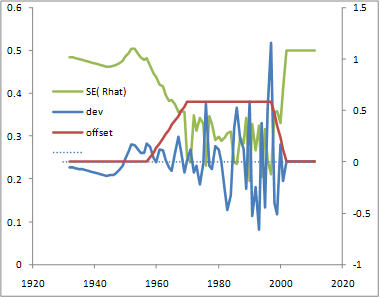
\includegraphics{10_bias}
\end{center}

Because the quantity and quality of data varies during a time series, SS allows the user to control the rate at which the offset is ramped in during the early, data-poor years, and then ramped back to zero for the forecast years.
On output to report.sso, SS calculates the mean bias adjustment during the early and main eras and compares it to the RMSE of estimated recruitment deviations.  A warning is generated if the RMSE is small and the bias adjustment is larger than 2.0 times the ratio of $rmse^2$ to $sigmaR^2$.

In MCMC mode, the model still draws recruitment deviations from the lognormal distribution, so the full offset is used such that the expected mean recruitment from this lognormal distribution will stay equal to the mean from the spawner-recruitment curve. When SS reaches the MCMC and MCEVAL phases, all bias adjustment values are set to 1.0 for all active recruitment deviations because the model is now re-sampling from the full lognormal distribution of each recruitment.

\subsubsection{Recruitment Autocorrelation}
The autocorrelation parameter is implemented.  It is not performance tested and it has no effect on the calculation of the offsets described in the section above.

\subsubsection{Recruitment Cycle}
When SS is configured such that seasons are modeled as years, the concept of season within year disappears.  However, there may be reason to still want to model a repeating pattern in expected recruitment to track an actual seasonal cycle in recruitment.  If the recruitment cycle factor is set to a positive integer, this value is interpreted as the number of time units in the cycle and this number of full parameter lines will be read.  The cyclic effect is modeled as an exp(p) factor times R0, so a parameter value of 0.0 has nil effect.  In order to maintain the same number of total recruits over the duration of the cycle, a penalty is introduced so that the cumulative effect of the cycle produces the same number of recruits as Ncycles * R0.  Because the cyclic factor operates as an exponential, this penalty is different than a penalty that would cause the sum of the cyclic factors to be 0.0.  This is done by adding a penalty to the parameter likelihood, where:
\begin{equation}
	\begin{split}
				   X & = \sum(e^p)  \\
				   Y & = Ncycle  \\
				   Penalty & = 100000*(X-Y)^2
	\end{split}
\end{equation}

\subsubsection{Initial Age Composition}
A non-equilibrium initial age composition is achieved by setting the first year of the recruitment deviations before the model start year.  These pre-start year recruitment deviations will be applied to the initial equilibrium age composition to adjust this composition before starting the time series.  The model first applies the initial F level to an equilibrium age composition to get a preliminary N-at-age vector and the catch that comes from applying the F's to that vector, then it applies the recruitment deviations for the specified number of younger ages in this vector.  If the number of estimated ages in the initial age composition is less than Nages, then the older ages will retain their equilibrium levels.  Because the older ages in the initial age composition will have progressively less information from which to estimate their true deviation, the start of the bias adjustment should be set accordingly.

\subsection{Fishing Mortality Method}
There are  three methods available for calculation of fishing mortality.  These are:  Pope's approximation, continuous F with each F as a model parameter, and a hybrid method that does a Pope's approximation to provide initial values for iterative adjustment of the continuous F values to closely approximate the observed catch.  With the hybrid method, the final values are in terms of continuous F, but do not need to be specified as full parameters.  In a 2 fishery, low F case, the hybrid method is just as fast as the Pope approx. and produces identical result.  When F is very high, the problem becomes quite stiff for Pope's and the hybrid method so convergence may slow.  It may  be better to use F option 2 (continuous F as full parameters) in these high F cases.  F as parameter is also preferred for situations where catch is known imprecisely and you are willing to accept a solution in which the final F values do not reproduce the input catch levels exactly.  For the F as parameter approach, there is an option to do early phases using hybrid, then switch to F as parameter in later phases and transfer the hybrid F values to the parameter initial values.\\
Option 1 (Pope's approx) still exists, but it is recommended to switch to option 3.


\begin{longtable}{p{1cm} p{3cm} p{11cm}}
	\multicolumn{3}{l}{Control file continued:}\\
	\hline
	\multicolumn{2}{l}{Typical Value} & Description and Options\Tstrut\Bstrut\\
	\hline
	\endfirsthead

	\hline
	\multicolumn{2}{l}{Typical Value} & Description and Options\Tstrut\Bstrut\\
	\hline
	\endhead

	\hline
	\endfoot
	\endlastfoot

	0.2 \Tstrut & & F ballpark\\
	    & & This value is compared to the sum of the F's for the specified year.  The sum is over all seasons and areas.  In older versions of SS, the lambda was automatically set to 0.0 in the final phase, the user now has control over whether to reduce the \hyperlink{Lambdas}{lambda} in later phases.\Bstrut\\
   \hline

	-1990\Tstrut & & F ballpark year\\
	      & & Negative value disable F ballpark.\Bstrut\\
   \hline

	3 \Tstrut & & F Method \\
	   & & 1 = Pope's (discrete), \\
	   & & 2 = Baranov (continuous) F as a parameter, \\
	   & & 3 = Hybrid F (recommended).\Bstrut\\
   \hline

   2.9 \Tstrut & & Maximum F \\
       & & This maximum is applied within each season and area.   A value of 0.9 is recommended for F method 1, and a value of about 4 is recommended for F method 2 and 3. \Bstrut\\
   \hline

   \multicolumn{3}{l}{COND: F method = 1, no additional input for Pope's approximation.}\Tstrut\Bstrut\\
   \hline

   \multicolumn{3}{l}{COND: F method = 2: }\Tstrut\\
   & 0.10  1  1 & Initial F value, Phase, N F detail setup lines to read. Starting value for each F.  Initializing value for each F parameter.\\
   &  & For phases prior to the phase of the F value becoming active,  SS will use the hybrid option and the F values so calculated become the starting values for the F parameters when this phase is reached.\\		   
   \multicolumn{3}{l}{If F method = 2 and N for F detail is > 0}\Tstrut\\
   \multicolumn{2}{l}{1 1980 1 0.20 0.05 4} & fleet, year, season, F, SE, phase - these values override the catch se values in the data file and the overall starting F value and phase read just above.\Bstrut\\
   \hline

   \multicolumn{3}{l}{COND: Fmethod = 3}\Tstrut\\
   & 4 & Number of tuning iterations in hybrid method. A value of 2 or 3 is sufficient with a single fleet and low Fs.  A value of 5 or so may be needed to match the catch near exactly when there are many fleets and high F. \Bstrut\\
   \hline
\end{longtable}

\subsubsection{Initial Fishing Mortality}
Read a short parameter setup line for each fishery.  The parameters are the fishing mortalities for the initial equilibrium.  Do not try to estimate parameters for fisheries with zero initial equilibrium catch.  If there is catch, then give a starting value greater than zero and it generally is best to estimate the parameter in phase 1.

In SS3.30, the initial equilibrium year has explicit seasons, so the needed initial F values will also be by season.  Initial F values are only needed for fleet/seasons that have catch.  So if no fleet/season combo has catch, then no parameters are needed.

It is possible to use the initial F method to achieve an estimate of the initial equilibrium Z in cases where the initial equilibrium catch is unknown.  To do this:
\begin{itemize}
	\item Include a positive value for the initial equilibrium catch;
	\item Set the lambda for the logL for initial equilibrium catch to a nil value (hence causing SS to ignore the lack of fit to the input catch level;
	\item Allow the initial F parameter to be estimated.  It will be influenced by the early age and size comps which should have some information about the early levels of Z.
\end{itemize}

\hypertarget{Qsetup}{}
\subsection{Catchability}
Catchability is the scaling factor that relates a model quantity to the expected value for some type of data (index).  Typically this is used to converted selected numbers or biomass for a fleet into the expected value for a survey or CPUE by that fleet.  In SS, the concept has been extended so that, for example, a time series of an environmental factor could be treated as a survey of the time series of deviations for some parameter.  This flexibility means that a family of link functions beyond simple proportionality is needed.

For each fishery and survey with an index, enter a row with the entries as described below:

\begin{enumerate}
	\item Fleet Number
	\item Link type or index of dev vector: An assumed functional form between Q, the expected value, and the survey observation.
	\begin{enumerate}
		\item 1 = simple Q, proportional assumption about Q: $y=q*x$.
		\item 2 = mirror simple Q, 1 mirrored parameter.  
		\item 3 = Q with power, 2 parameters establish a parameter for non-linearity in survey-abundance linkage.  Assumes proportional with offset and power function: $y=qx^c$ where $q = exp(lnQ_base))$ thus the $c$ is not related to expected biomass but vulnerable biomass to Q.  Therefore, $c$ $<$ 0 leads to hyper-stability and $c > 0$ leads to hyper-depletion.
		\item 4 = mirror Q with offset (2 parameter lines required). The mirrored Q with offset for with be reported as base Q + offset value. Mirror in Q must refer to a lower number fleet relative to the fleet with the mirrored Q. See \hyperlink{MirrorQoffset}{mirrored Q with offset} below for example set up.
		\item If the parameter is for an index of a dev vector (index units = 35), use this column to enter the index of the dev vector to which the index is related
	\end{enumerate}
	\item Extra input for link (i.e. mirror fleet)
	\begin{enumerate}
		\item >0 = mirror the Q from another (lower numbered survey designated by abs(value))
	\end{enumerate}
	\item Do extra SD
	\begin{enumerate}
		\item 0 = skip (typical)
		\item 1 = estimate a parameter that will contain an additive constant to be added to the input standard deviation of the survey variability.  This extra SD approach accomplishes the same thing in principle as the older code, but may not give exactly the same answer as the older code.  The newer code for extra SD estimation is recommended.
	\end{enumerate}
	\item Bias adjustment
	\begin{enumerate}
		\item 0 = no bias adjustment applied
		\item 1 = apply bias adjustment
	\end{enumerate}
	\item Q float
	\begin{enumerate}
		\item 0 = no float (parameter is estimated)
		\item 1 = float (analytical solution is used, but parameter line still required)
		\item Additional information regarding the use of and appropriate application of float in Q can be found in the \hyperlink{FloatQ}{Float Q} section below.
	\end{enumerate}
\end{enumerate}



\begin{longtable}{p{2cm} p{2cm} p{2cm} p{2cm} p{2cm} p{1.3cm} p{2.3cm}}
	\multicolumn{7}{l}{For a setup with a single survey, the Q setup matrix could be:}\\
	\hline
	Fleet \Tstrut & Link & Link & Extra  & Bias   &   & \\
	Num.          & Type & Info & SD     & Adjust & Float  & Label\Bstrut\\
	\hline
	3 & 1 & 0 & 1 & 1 & 0 & \#Survey  \Tstrut\\
	-9999 & 0 & 0 & 0 & 0 & 0 & \#End Read \Bstrut\\
	\hline
\end{longtable}


\begin{longtable}{p{1cm} p{1cm} p{1cm}  p{1.5cm}  p{1.5cm} p{1.5cm}  p{1.75cm}  p{4cm} }
	\hline
	LO \Tstrut & HI & INIT & <other entries> & PHASE & <other entries> & Block Fxn & Parameter Label\Bstrut\\
	\hline
	\endfirsthead

	\hline
	LO \Tstrut & HI & INIT & <other entries> & PHASE & <other entries> &Block Fxn & Parameter Label\Bstrut\\
	\hline
	\endhead

	\hline
	\endfoot
	\endlastfoot

	-5 & 5   & -0.12 & \multicolumn{1}{c}{...} & 1  & \multicolumn{1}{c}{...} & 0  & \#Survey1 LnQ base\Tstrut\\
	0  & 0.5 & 0.1   & \multicolumn{1}{c}{...} & -1 & \multicolumn{1}{c}{...} & 0  & \#Survey1 Extra SD\Bstrut\\
	\hline
\end{longtable}

If the Q base parameter specifies that it is time-varying by the annual dev method, short parameter lines to specify the specifications of the deviation vector come after all the base Q parameters.

\hypertarget{MirrorQoffset}{}
\subsubsection{Mirrored Q with offset}
Below is an example setup for fleets with a mirrored Q and offset from another fleet:
\begin{longtable}{p{2cm} p{2cm} p{2cm} p{2cm} p{2cm} p{1.3cm} p{2.3cm}}
	\multicolumn{7}{l}{For a setup with a single survey, the Q setup matrix could be:}\\
	\hline
	Fleet \Tstrut & Link & Link & Extra  & Bias   &   & \\
	Num.          & Type & Info & SD     & Adjust & Float  & Label\Bstrut\\
	\hline
	1 & 1 & 0 & 1 & 0 & 0 & \#Fleet 1  \Tstrut\\
	2 & 4 & 2 & 0 & 0 & 0 & \#Fleet 2  \Tstrut\\
	-9999 & 0 & 0 & 0 & 0 & 0 & \#End Read \Bstrut\\
	\hline
\end{longtable}


\begin{longtable}{p{1cm} p{1cm} p{1cm}  p{1.5cm}  p{1.5cm}  p{1.5cm} p{1.75cm}  p{4cm} }
	\multicolumn{8}{l}{A long parameter line is expected for each link parameter (i.e. Q) and for the}\\
	\hline
	LO \Tstrut & HI & INIT & <other entries> &  PHASE & <other entries> & Block Fxn & Parameter Label\Bstrut\\
	\hline
	\endfirsthead
	
	\hline
	\endfoot
	\endlastfoot
	
	-7 & 5   & 0.51 & \multicolumn{1}{c}{...} & 1  & \multicolumn{1}{c}{...} & 0  & \#Fleet 1 LnQ base\Tstrut\\
	0  & 0.5 & 0.1  & \multicolumn{1}{c}{...} & -1 & \multicolumn{1}{c}{...} & 0  & \#Fleet 1 Extra SD\Tstrut\\
	-7 & 5   & -6   & \multicolumn{1}{c}{...} & -1 & \multicolumn{1}{c}{...} & 0  & \#Fleet 2 LnQ base\Bstrut\\
	-8 & 5   & -7   & \multicolumn{1}{c}{...} & -1 & \multicolumn{1}{c}{...} & 0  & \#Fleet 2 Mirror Q  offset\Bstrut\\
	\hline
\end{longtable}

\hypertarget{FloatQ}{}
\subsubsection{Float Q}
The use and development of float in Q has evolved over the life of SS. The original difference in earlier versions of SS (early SS v.3.24 versions and before) is that with Q "floated" the units of the survey or fishery CPUE are treated as dimensionless so the Q is adjusted within each model iteration to maintain a mean difference of 0.0 between observed and expected (usually in log space).  But with Q as a parameter one gets the ability to interpret the absolute scaling of Q and put a prior on it to help guide the model solution.  Also, with Q as a parameter the code allows for Q to be time-varying.

Then midway through the evolution of the SS v.3.24 code lineage a new Q option was introduced based on user recommendations.  This option allowed Q to float and to compare the resulting Q value to a prior, hence the information in that prior would pull the model solution in direction of a floated Q that came close to the prior.

Currently, in 3.30, that float with prior capability is fully embraced.  All fleets that have any survey or CPUE options need to have a catchability specification and get a base Q parameter in the list.  Any of these Q's can be either:

\begin{itemize}
	\item Fixed: by not floating and not estimating.

	\item Floating: not estimated as an active parameter, set phase to negative, and not capable of being time-varying.  Can have a prior, or not.  Future versions of SS may allow Q to be time-varying and then rescaling that Q vector according to the float logic but this is not yet currently implemented.

	\item Estimated as active parameter: so not floating. Can be time-varying and can have a prior.
\end{itemize}

Q relates the units of the survey or CPUE to the population abundance, not the population density per unit area.  But many surveys and most fishery CPUE is a proportional to mean fish density per unit area.  This does not have any impact in a one area model because the role of area is absorbed into the value of Q.  In a multi-area model, one may want to assert that the relative difference in CPUE between two areas is informative about the relative abundance between the areas.   However, CPUE is a measure of fish density per unit area, so one may want to multiply CPUE by area before putting the data into SS so that asserting the same Q for the two areas will be informative about relative abundance.

In SS v.3.30.13, a new catchability option has been added that allows Q to be mirrored and to add an offset to ln(Q) of the primary area when calculating the ln(Q) for the dependent area.  The offset is a parameter and, hence, can be estimated and have a prior.  This option allows the CPUE data to stay in density units and the effect of relative stock area is contained in the value of the ln(Q) offset.


\subsubsection{Conversion issues between SS v.3.24 and v.3.30}
In SS v.3.24 it was common to use the deviation approach and this deviation approach in SS v.3.24 was implemented as if it was survey specific blocks.  In some cases, only one year's deviation was made active in order to implement, in effect, a block for Q.  sstrans.exe cannot convert this, but an analogous approach is available in SS v.3.30 because true blocks can now be used, as well as env links and annual deviations.  Also note that deviations in SS v.3.24 were survey specific (so no parameter for years with no survey).  But in SS v.3.30, deviations are always year-specific, so you might have a deviation created for a year with no survey.

\subsection{Selectivity and Discard}
For each fleet and survey, read a definition line for size selectivity and retention.  The four values read from each line are:

\myparagraph{Pattern}
Valid length selectivity pattern code.

\begin{itemize}
	%\item[Discard]\hfill\\
	\item Discard \hypertarget{DomeRetention}{(0/1/2/3/4 or -index)} If value is 1, then program will read 4 retention parameters after reading the specified number of selectivity parameters and all discarded fish are assumed dead.  If the value is 2, then the program will read 4 retention parameters and 4 discard mortality parameters.  If the value is 3, then no additional parameters are read and all fish are assumed discarded and dead. If the value is 4, then the program will read 7 retention parameters (for dome-shaped retention) and 4 discard mortality parameters.  If the value is a negative number, then it will mirror the retention and discard mortality pattern of the lower numbered fleet.

%	\item[Male]\hfill\\
	\item Male (0/1/2/3/4)  If value is 1, then program will read 4 additional parameters to define the male selectivity relative to the female selectivity.  Anytime the male selectivity is caused to be greater than 1.0; the entire male/female matrix of selectivity values is scaled by the max so that the realized max is 1.0.  Hopefully this does not cause gradient problems.  If the value is 2, then the main selectivity parameters define male selectivity and female selectivity is estimated as an offset from male selectivity.  This alternative is preferable if female selectivity is less than male selectivity.  The option 3 is only available if the selectivity pattern is 1, 20, or 24 and it causes the male selectivity parameters to be offset from the female parameters, rather than the male selectivity being an offset from the female selectivity.

%	\item[Special]\hfill\\
	\item Special (0/value).  This value is used in different ways depending on the context.  If the selectivity type is to mirror another selectivity type, then put the index of that source fleet or survey here.  It must refer to a lower numbered fleet/survey.  If the selectivity type is 6 (linear segment), then put the number of segments here.  If the selectivity type is 7, then put a 1 here to keep selectivity constant above the mean average size for old fish of morph 1.
\end{itemize}
%\end{description}

For each fleet and survey, read a definition line for age selectivity.  The 4 values to be read are the same as for the size-selectivity.  However, the retention value must be set to 0.

\begin{center}
	\begin{longtable}{p{2cm} p{2cm} p{2cm} p{2cm} p{6.5cm} }
		\hline
		\multicolumn{5}{l}{Example Setup for Size Selectivity:}\Tstrut\\
		Pattern & Discard & Male & Special & Label \Bstrut\\
		\hline
		1  & 2 & 0 & 0 & \#Fishery1\Tstrut\\
		1  & 0 & 0 & 0 & \#Survey1\\
		0  & 0 & 0 & 0 & \#Survey2\Bstrut\\
		\hline

		\multicolumn{5}{l}{Age Selectivity Types:}\Tstrut\\
		Pattern & Discard & Male & Special & Label \Bstrut\\
		\hline
		11  & 0 & 0 & 0 & \#Fishery1\Tstrut\\
		11  & 0 & 0 & 0 & \#Survey1\\
		11  & 0 & 0 & 0 & \#Survey2\Bstrut\\
		\hline
	\end{longtable}
\end{center}

\subsubsection{Reading the Selectivity and Retention Parameters}
Read the required number of parameter setup lines as specified by the definition lines above.  The complete order of the parameter setup lines is:
\begin{enumerate}
	\item Size selectivity for fishery 1
	\item Retention for fishery 1 (if discard specified)
	\item Discard Mortality for fishery 1 (if discard specified)
	\item Male offsets for size selectivity for fishery 1 (if offsets used)
	\item <repeat for additional fleets and surveys>
	\item Age selectivity for fishery 1
	\item Male offsets for age selectivity for fishery 1 (if offsets used)
	\item <repeat for additional fleets and surveys>.
\end{enumerate}


\begin{longtable}{p{1cm} p{1cm} p{1cm}  p{1.5cm}  p{2.9cm}  p{1.9cm}  p{4.2cm}}
	\multicolumn{7}{l}{The list of parameters to be read from the above setup would be:}\\
	\hline
	LO \Tstrut & HI & INIT & PRIOR &  <other entries> & Block Fxn & Parameter Label\Bstrut\\
	\hline
	\endfirsthead

	\hline
	LO \Tstrut & HI & INIT & PRIOR & <other entries> & Block Fxn & Parameter Label\Bstrut\\
	\hline
	\endhead
		
	19    & 80   & 53.5 & 50  & \multicolumn{1}{c}{...}  & 0   & \#SizeSel p1 fishery 1\Tstrut\\
	0.01  & 60   & 18.9 & 15  & \multicolumn{1}{c}{...}  & 0   & \#SizeSel p2 fishery 1 \\
	20    & 70   & 38.6 & 40  & \multicolumn{1}{c}{...}  & 0   & \#Retain p1 fishery 1\\
	0.1   & 10   & 6.5  & 1   & \multicolumn{1}{c}{...}  & 0   & \#Retain p2 fishery 1\\
	0.001 & 1    & 0.98 & 1   & \multicolumn{1}{c}{...}  & 0   & \#Retain p3 fishery 1\\
	-10   & 10   & 1    & 0   & \multicolumn{1}{c}{...}  & 0   & \#Retain p4 fishery 1\\
	0.1   & 1    & 0.6  & 0.6 & \multicolumn{1}{c}{...}  & 0   & \#DiscMort p1 fishery 1\\
	-2    & 2    & 0    & 0   & \multicolumn{1}{c}{...}  & 0   & \#DiscMort p2 fishery 1\\
	20    & 70   & 40   & 40  & \multicolumn{1}{c}{...}  & 0   & \#DiscMort p3 fishery 1\\
	0.1   & 10   & 1    & 1   & \multicolumn{1}{c}{...}  & 0   & \#DiscMort p4 fishery 1\\
	19    & 80   & 53.5 & 50  & \multicolumn{1}{c}{...}  & 0   & \#SizeSel p1 survey 1\\
	0.01  & 60   & 18.9 & 15  & \multicolumn{1}{c}{...}  & 0   & \#SizeSel p2 survey 1 \\
	0     & 40   & 0    & 5   & \multicolumn{1}{c}{...}  & 0   & \#AgeSel p1 fishery 1\\
	0     & 40   & 40   & 5   & \multicolumn{1}{c}{...}  & 0   & \#AgeSel p2 fishery 1\\
	0     & 40   & 0    & 5   & \multicolumn{1}{c}{...}  & 0   & \#AgeSel p1 survey 1\\
	0     & 40   & 40   & 5   & \multicolumn{1}{c}{...}  & 0   & \#AgeSel p2 survey 1\\
	0     & 40   & 0    & 5   & \multicolumn{1}{c}{...}  & 0   & \#AgeSel p1 survey 2\\
	0     & 40   & 0    & 5   & \multicolumn{1}{c}{...}  & 0   & \#AgeSel p2 survey 2\Bstrut\\
	\hline
\end{longtable}



\subsubsection{Selectivity Patterns}
The currently defined selectivity patterns, and corresponding required number of parameters, are:


\begin{longtable}{p{2cm} p{3cm} p{10cm}}
	\multicolumn{3}{c}{SIZE BASED SELECTIVITY}\Bstrut\\	
	\endfirsthead

	\hline
	Pattern & N Parameters & Description \Tstrut\Bstrut\\
	\hline
	\endhead

	\hline
	\endfoot
	\endlastfoot

	\hline
		
	Pattern & N Parameters & Description \Tstrut\Bstrut\\
	\hline
	0 \Tstrut& 0 & Selectivity = 1.0 for all sizes. \\
	1 \Tstrut& 2 & Logistic selectivity.\\
	2 \Tstrut& 8 & Discontinued: Double logistic with defined peak (uses IF joiners). Use pattern 8 instead.\\
	3 \Tstrut& 6 & Discontinued \\
	4 \Tstrut& 0 & Discontinued: Set size selectivity equal to female fecundity. Use \hyperlink{SpecialSurvey}{special survey pattern 30} located in the index section within the data file instead.\\
	5 \Tstrut& 2 & Mirror another selectivity. The two parameters select bin range.\\
	6 \Tstrut& 2 + special value & Non-parametric \\
	7 \Tstrut& 8 & Discontinued: Double logistic with defined peak, uses smooth joiners; special = 1 causes constant selectivity above Linf for morph 1.  Use pattern \#8.\\
	8 \Tstrut& 8 & Double logistic, with defined peak, uses smooth joiners; special=1 causes constant selectivity above $L_{inf}$ for morph 1.  \\
	9 \Tstrut& 6 & Simple double logistic with no defined peak.\\
	15 \Tstrut& 0 & Mirror another selectivity (same as for age selectivity).\\
	21 \Tstrut& 1 + special value  & Non-parametric size selectivity\\
	22 \Tstrut& 4 & Double normal; similar to CASAL.\\
	23 \Tstrut& 6 & Same as the double normal pattern 24 except the final selectivity is now directly interpreted as the terminal selectivity value. Cannot be used with Pope's F method because maximum selectivity may be greater than 1.\\
	24 \Tstrut& 6 & Double normal with defined initial and final selectivity level – Recommended option.  Test using SELEX-24.xls. \\
	25 \Tstrut& 3 & Exponential-logistic. \\
	27 \Tstrut& 3 + 2*N nodes & Cubic spline with N nodes. \\
	42 \Tstrut& 5 + 2*x & Selectivity pattern 27 but with 2 additional scaling parameters. \\
	43 \Tstrut& 4 + x & Selectivity pattern 6 but with 2 additional scaling parameters.\Bstrut\\
	\hline
\end{longtable}




\begin{longtable}{p{2cm} p{3cm} p{10cm}}
	\multicolumn{3}{c}{AGE BASED SELECTIVITY}\\
	\endfirsthead

	\hline
	Pattern & N Parameters & Description \Tstrut\Bstrut\\
	\hline
	\endhead

	\hline
	\endfoot
	\endlastfoot
	
	\hline
	Pattern & N Parameters & Description  \Tstrut\Bstrut\\
	\hline
	0  \Tstrut& 0 & Selectivity = 1.0 for ages 0+.\\
	10 \Tstrut& 0 & Selectivity = 1.0 for all ages beginning at age 1.  If it is desired that age-0 fish be selected, then use pattern \#11 and set minimum age to 0.0. \\
	11 \Tstrut& 2 & Selectivity = 1.0 for a specified age range.\\
	12 \Tstrut& 2 & Logistic selectivity.\\
	13 \Tstrut& 8 & Double logistic, IF joiners.  Use discouraged.  Use pattern 18 instead.\\
	14 \Tstrut& nages + 1 & Separate parameter for each age (empirical), value at age is $\frac{1}{1+exp(-x)}$. \\
	15 \Tstrut& 0 & Mirror another age-specific selectivity pattern.\\
	16 \Tstrut& 2 & Coleraine single Gaussian\\
	17 \Tstrut& nages + 1 & Empirical as a random walk from previous age.  For all ages in the population beginning with Amin = 1 for the fishery and 2 for the survey, there is a corresponding set of selectivity parameters for each fleet, $p_a$. \\
	18 \Tstrut& 8 & Double logistic, with defined peak, uses smooth joiners.  \\
	19 \Tstrut& 6 & Simple double logistic with no defined peak.\\
	20 \Tstrut& 6 & Double normal with defined initial and final level.  Recommended option. Test using SELEX-24.xls.\\
	26 \Tstrut& 3 & Exponential logistic.\\
	27 \Tstrut& 3 + 2*N nodes & Cubic spline in age based on N nodes.\\
	41 \Tstrut& 2 + nages + 1 & Selectivity pattern 17 but with 2 additional scaling parameters. \\
	42 \Tstrut& 5 + 2*N nodes & Selectivity pattern 27 but with 2 additional scaling parameters. \\
	44 \Tstrut& 4 + nages & Similar to age selectivity pattern 17 but with separate parameters for males and with revised controls. \\
	45 \Tstrut& 4 + nages & Similar to age selectivity pattern 14 but with separate parameters for males and with revised controls.\Bstrut\\
	\hline
\end{longtable}


%\begin{description}
\myparagraph{Special Selectivity Options}
%	\item[Special Selectivity Options]\hfil\\
Special selectivity options (type 30 in size based selectivity) are no longer specified within the control file. Specifying the use of one of these selectivity types is now done within the data file by selecting the survey "units" (see the section on \hyperlink{IndexUnits}{Index units}).	
%\end{description}

\subsubsection{Selectivity Pattern Details}
%\begin{description}
\myparagraph{Pattern 1 (size) and 12 (age) - Simple Logistic}
%	\item[Pattern 1 (size) and 12 (age) - Simple Logistic]\hfill\\
Within SS logistic selectivity for the primary sex (if selectivity varies by sex) is formulated as:
	\begin{equation}
	S_l = \frac{1.0}{1+exp(-ln(19)(L_l - p1)/p2)}
	\end{equation}
where $L_l$ is the length bin.  If age based selectivity is selected then the length bin is replaced by the age vector. If sex specific selectivity is specified the non-primary sex the p1 and p2 parameters are estimated as offsets.  Note that with a large p2 parameter, selectivity may not reach 1.0 at the largest size bin. The parameters are:
\begin{itemize}
	\item p1 - size/age at inflection
	\item p2 - width for 95\% selection; a negative width causes a descending curve.
\end{itemize}
%\end{description}


%\begin{description}
\myparagraph{Pattern 5 (size) - Mirror Selectivity}
%	\item[Pattern 5 (size) - Mirror Selectivity]\hfil\\
Two parameters select the min and max bin number (not min max size) of the source pattern.  If first parameter has value <=0, then interpreted as a value of 1 (e.g. first bin).  If second parameter has value <=0, then interpreted as nlength (e.g. last bin). The source pattern must have a lower type number
%\end{description}	


%\begin{description}
\myparagraph{Pattern 6 (size) - Non-parametric Selectivity}
%	\item[Pattern 6 (size) - Non-parametric Selectivity]\hfil\\
Non-parametric size selectivity uses a set of linear segments.  The first way point is at Length = p1 and the last way point is at Length = p2.  The total number of way points is specified by the value of the Special factor in the selectivity set-up, so the N intervals is one less than the number of way points  Intermediate way points are located at equidistant intervals between p1 and p2.  Parameters 3 to N are the selectivity values at the way points, entered as logistic, e.g. $1/(1+exp(-x))$.  Ramps from 10cm to p3 if L<p1.  Constant at Np if L>p2.  Note that prior to version 3.03 the way points were specified in terms of bin number, rather than length.
%\end{description}

%\begin{description}
\myparagraph{Pattern 8 (size) and 18 (age) - Double Logistic}
%	\item[Pattern 8 (size) and 18 (age) - Double Logistic]\hfil
	\begin{itemize}
		\item  p1 – PEAK:  size (age) for peak. Should be an integer and should be at bin boundary and not estimated.  But options 7 and 18 may allow estimation.
		\item p2 – INIT:  selectivity at length bin=1 (minL) or age=0.
		\item p3 – INIT:  selectivity at length bin=1 (minL) or age=0. A logit transform $(1/(1+exp(-x))$ is used so that the transformed value will be between 0 and 1.  So a p1 value of –1.1 will be transformed to 0.25 and used to set the selectivity equal to 0.5 at a size (age) equal to 0.25 of the way between minL and PEAK. 
		\item p4 – SLOPE1:  log(slope) of left side (ascending) selectivity.
		\item p5 – FINAL:  logit transform for selectivity at maxL (or maxage).
		\item p6 – INFL2:  logit transform for size(age) at right side selectivity equal to half way between PEAK+PEAKWIDTH and maxL (or max age).
		\item p7 – SLOPE2:  log(slope) of right side (descending) selectivity
		\item p8 – PEAKWIDTH:  in width of flattop.
	\end{itemize}
%\end{description}

%\begin{description}
\myparagraph{Pattern 14 (age) - Revise Age}
%	\item[Pattern 14 (age) - Revise Age]\hfil\\
Age-selectivity pattern 14 to allow selectivity-at-age to be the same as selectivity at the next younger age.  When using this option, the range on each parameter should be approximately -5 to 9 to prevent the parameters from drifting into extreme values with nil gradient. SS calculates the age-based selectivity as where $a = 1$ to $a = Amax + 1$:
	\begin{equation}
		 \begin{split}
		 temp = 9 - max(p(a))\\
		S_a = \frac{1}{1+exp(-(p(a+1) + temp))}
		\end{split}
	\end{equation}	
%\end{description}

%\begin{description}
\myparagraph{Pattern 17 (age) - Random Walk}
%	\item[Pattern 17 (age) - Random Walk]\hfill\\
This selectivity pattern provides for a random walk in ln(selectivity).  For each age $a \geq A_{\text{min}}$, where $A_{\text{min}}$ is the minimum age for which selectivity is allowed to be non-zero, there is a selectivity parameter, $p_a$, controlling the changein selectivity from age $a-1$ to age $a$.
	
The selectivity at age $a$ is computed as
	\begin{equation}
	S_a = \exp (S'_a - S'_{\text{max}}),
	\end{equation}
where
	\begin{equation}
	S'_a = \sum_{i = A_{\text{min}}}^a p_i
	\end{equation}
and 
	\begin{equation}
	S'_{\text{max}} = \mbox{max} \{S'_a\}.
	\end{equation}
Selectivity is fixed at $S_a = 0$ for $a < A_{\text{min}}$. 
	
This formulation has the properties that the maximum selectivity equals 1, positive values of $p_a$ are associated with increasing selectivity between ages $a-1$ and $a$, and negative values are associated with decreasing selectivity between those ages and $p_a = 0$ gives constant selectivity.
	
The condition that maximum selectivity equals 1 results in one fewer degree of freedom than the number of estimated $p_a$. Therefore, at least one parameter should be fixed at an arbitrary value, typically $p_{A_{\text{min}}}=0$.
	
In typical usage:
	\begin{itemize}
		\item First parameter (for age 0) could have a value of -1000 so that the age 0 fish would get a selectivity of 0.0;
		\item 	Second parameter (for age 1) could have a value of 0.0 and not be estimated, so age 1 is the reference age against which subsequent changes occur;
		\item 	Next parameters get estimated values.  To assure that selectivity increases for the younger ages, the parameter min for these parameters could be set to 0.0 or a slightly negative value.
		\item If dome-shaped selectivity is expected, then the parameters for older ages could have a range with the max set to 0.0 so they cannot increase further.
		\item To keep selectivity at a particular age the same as selectivity at the next younger age, set its parameter value to 0.0 and not estimated.  This allows for all older ages to have the same selectivity.
		\item 	To keep a constant rate of change in selectivity across a range of ages, use the -999 flag to keep the same rate of change in ln(selectivity) as for the previous age.
		\item  Code for implementing random walk selectivity within SS can be found in \hyperlink{RandWalkSelex}{Appendix C}.
	\end{itemize}
%\end{description}

%\begin{description}
\myparagraph{Pattern 9 (size) and 19 (age) - Simple Double Logistic with no defined peak}
%\item[Pattern 9 (size) and 19 (age) - Simple Double Logistic with no defined peak]\hfil
	\begin{itemize}
		\item p1 - INFL1:  ascending inflection size (in cm)
		\item p2 – SLOPE1:  ascending slope
		\item p3 – INFL2:  descending inflection size (in cm)
		\item p4 – SLOPE2:  descending slope
		\item p5 – first BIN: bin number for the first bin with non-zero selectivity (must be an integer bin number, not a size)
		\item p6 – offset:  enter 0 if P3 is independent of P1; enter 1 if P3 is an offset from P1
	\end{itemize}
%\end{description}

%\begin{description}
\myparagraph{Pattern 22 (size) - Double Normal with Plateau}
%	\item[Pattern 22 (size) - Double Normal with Plateau]\hfil
	\begin{itemize}
		\item p1 – PEAK1:  beginning size for the plateau (in cm)
		\item p2 – PEAK2:  ending size for the plateau.  Calculated as a fraction of the distance between PEAK1 and 99\% of the lower edge of the last size bin in the model.  Transformed as (1/(1+exp(-p2)).   So a value of 0 results in PEAK2 being halfway between PEAK1 and 99\% of the last bin
		\item p3 – upslope:  ln(variance) on ascending side
		\item p4 – downslope:  ln(variance) on descending side
	\end{itemize}
%\end{description}

%\begin{description}
\myparagraph{Pattern 23 (size) and 24 (size) - Double Normal Selectivity}	%\item[Pattern 23 (size) and 24 (size) - Double Normal Selectivity]\hfil
	\begin{itemize}
		\item p1 – PEAK:  beginning size for the plateau (in cm)
		\item p2 – TOP:  width of plateau, as logistic between PEAK and MAXLEN
		\item p3 – ASC-WIDTH:  parameter value is ln(width)
		\item p4 – DESC-WIDTH:  parameter value is ln(width)
		\item p5 – INIT:  selectivity at first bin, as logistic between 0 and 1.
		\item p6 – FINAL: selectivity at last bin, as logistic between 0 and 1.  (for pattern 24) or
		\item p6 – FINAL: selectivity at last bin, as absolute value, so can be >1.0.  (for pattern 23).  Warning:  Do not allow this value to go above 1.0 if the F\_method uses Pope’s approximation.  OK to go above 1.0 when F is in exponential form.  When this parameter is above 1.0, the overall selectivity pattern will have an intermediate plateau at 1.0 (according to peak and top), then will ascend further to the final value.
	\end{itemize}
	
Notes for Double Normal Selectivity:
	\begin{itemize}
		\item See spreadsheet SELEX-24.xls for parameterization example.
		\item For the initial selectivity parameter (parameter 5)
		\begin{itemize}
			\item -999 or –1000:   ignore the initial selectivity algorithm and simply decay the small fish selectivity according to P3,
			\item < -1000:  ignore the initial selectivity algorithm as above and then set selectivity equal to 1.0e-06 for size bins 1 through bin =  -1001 –value.  So a value of –1003 would set selectivity to a nil level for bins 1 through 2 and begin using the modeled selectivity in bin 3.
		\end{itemize}
		\item For the final selectivity parameter (parameter 6)
		\begin{itemize}
			\item -999 or –1000:   ignore the final selectivity algorithm and simply decay the large fish selectivity according to parameter 4,
			\item <-1000:  set selectivity constant for bins greater than bin number =  -1000 – value.
		\end{itemize}
	\end{itemize}
Selectivity pattern 24, double normal, showing sub-functions and steep logistic joiners:
	\begin{center}
		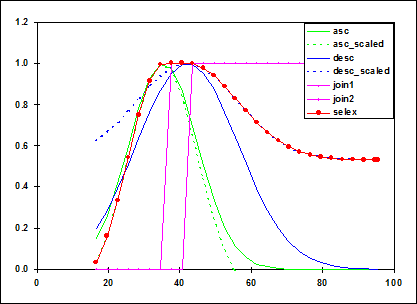
\includegraphics{DoubleNormal}
	\end{center}

\myparagraph{Pattern 15 (age) - Mirror}

No parameters.  Whole age range is mirrored from a user-specified fleet.

\myparagraph{Pattern 16 - Gaussian (similar to Coleraine)}

	\begin{itemize}
		\item p1 – age below which selectivity declines
		\item p2 – scaling factor for decline
	\end{itemize}


\myparagraph{Pattern 9 (size) and 19 (age) - Simple Double Logistic}

	\begin{itemize}
		\item p1 – ascending inflection age/size
		\item p2 – ascending slope
		\item p3 – descending inflection age/size
		\item p4 – descending slope
		\item p5 – age or size at first selection; this is a specification parameter, so must not be estimated.  Enter integer that is age for pattern 19 and is bin number for pattern 9
		\item p6 – (0/1)  where a value of 0 causes the descending inflection to be a standalone parameter, and a value of 1 causes the descending inflection to be interpreted as an offset from the ascending inflection.  This is a specification parameter, so must not be estimated.
	\end{itemize}
	A value of 1.0e-6 is added to the selectivity for all ages, even those below the minage.\\
%\end{description}

%\begin{description}
\myparagraph{Pattern 25 (size) and 26 (age) - Exponential logistic}
%	\item[Pattern 25 (size) and 26 (age) - Exponential logistic]\hfil
	\begin{itemize}
		\item p1 – ascending rate, min: 0.02, max: 1.0, reasonable start value:  0.1
		\item p2 – peak, as fraction of way between min size and max size.  Parameter min value:  0.01; max:  0.99; reasonable start value:  0.5
		\item p2 – minsize + p2*(maxsize-minsize)
		\item p3 – descending rate, min: 0.001, max: 0.5, reasonable start value:  0.01.  A value of 0.001 provides a nearly asymptotic curve.  Values above 0.2 provide strongly dome-shaped function in which the p3 and p1 parameters interact strongly.
	\end{itemize}
	\begin{equation}
	\frac{e^{p3*p1(p2'-size)}}{1-p3(1-e^{p1(p2'-size)})}
	\end{equation}
	Example: Exponential logistic selectivity with p1 = 0.30, p2 = 0.50, and p3 = 0.02:\\
	\begin{center}
		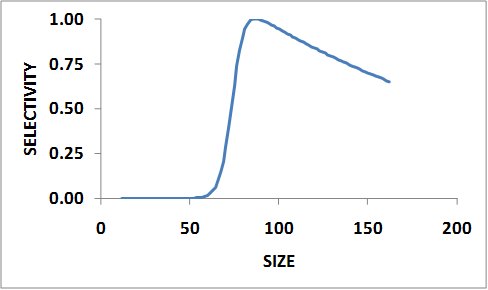
\includegraphics{ExpLogistic}
	\end{center}
%\end{description}

%\begin{description}
\myparagraph{Pattern 27 (size and age)- Cubic Spline}
%	\item[Pattern 27 (size and age)- Cubic Spline]\hfil\\
This selectivity pattern uses the ADMB implementation of the cubic spline function. This function requires input of the number of nodes, the positions of those nodes, the parameter values at those nodes, and the slope of the function at the first and last node.  In SS, the number of nodes is specified in the “special” column of the selectivity set-up.  The pattern number 27 is used to invoke cubic spline for size selectivity and for age selectivity; the input syntax is identical.
	
For a 3 node setup, the SS input parameters would be:
	\begin{itemize}
		\item p1 – 	code for initial set-up (0, 1 or 2) as explained below
		\item p2 – 	gradient at the first node (should be a small positive value)
		\item p3 – 	gradient at the last node (should be zero or a small negative value)
		\item p4-p6 – the nodes in units of cm; must be in rank order and inside of the range of the population length bins.  These must be held constant (not estimated, e.g. negative phase value) during a model run.
		\item  p7-p9 – the values at the nodes.  Units are ln(selectivity).
	\end{itemize}

Notes:
	\begin{itemize}
		\item There must be at least 3 nodes.
		\item One of these selectivity parameter values should be held constant so others are estimated relative to it.
		\item Selectivity is forced to be constant for sizes greater than the size at the last node
		\item The overall selectivity curve is scaled to have a peak equal to 1.0.
		\item Terminal nodes cannot be at the min or max population length bins.
	\end{itemize}
	
Code for implementing cubic spline selectivity within SS can be found in \hyperlink{CubicSpline}{Appendix C}.

	
The figure below compares a 3 node and a 6 node cubic spline with a 2 parameter logistic function.  In fitting these functions, the 2 cubic spline approaches fit slightly better than the logistic, presumably because the data were slightly indicative of a small dome in selectivity.
	\begin{center}
		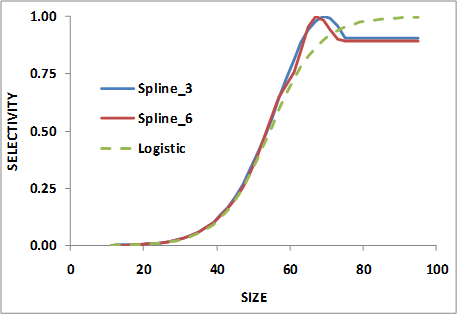
\includegraphics{CubicSpline}
	\end{center}
	
Auto-Generation of Cubic Spline Control File Set-Up: A New SS feature pioneered with the cubic spline function is a capability to produce more specific parameter labels and to auto-generate selectivity parameter setup.  The auto-generation feature is controlled by the first selectivity parameter value for each fleet that is specified to use the cubic spline.  There are 3 possible values for this setup parameter:
	\begin{itemize}
		\item 0: no auto-generation, process parameter setup as read.
		\item 1: auto-generate the node locations based on the specified number of nodes and on the cumulative size distribution of the data for this fleet/survey.
		\item 2: auto-generate the nodes and also the min, max, prior, init, and phase for each parameter.
	\end{itemize}
	
With either the auto-generate option \#1 or \#2, it still is necessary to include in the parameter file placeholder rows of values so that the init\_matrix command can input the current number of values because all selectivity parameter lines are read as a single matrix dimensioned as N parameters x 14 columns.  The read values of min, max, init, prior, prior type, prior stddev, and phase will be overwritten.
	
Cumulative size and age distribution is calculated for each fleet, summing across all samples and both sexes.  These distributions are output in echoinput.sso and in a new OVERALL\_COMPS section of report.sso.
	
When the nodes are auto-generated, the first node is placed at the size corresponding to the 2.5\% percentile of the cumulative size distribution, the last is placed at the 97.5\% percentile of the size distribution, and the remainder are placed at equally spaced percentiles along the cumulative size distribution.  These calculated node values are output into control.ss\_new.  So, the user could extract these nodes from control.ss\_new, edit them to desired values, then, insert them into the input control file.  Remember to turn off auto-generation in the revised control file.
	
When the complete auto-generation is selected, the control.ss\_new would look like the table below:	

\begin{longtable}{p{1cm} p{1cm} p{1cm} p{2.9cm}  p{1.9cm}  p{4.2cm}}
	\hline
	LO \Tstrut & HI & INIT  &  <other entries> & Block Fxn & Parameter Label\Bstrut\\
	\hline
	\endfirsthead

	\hline
	LO \Tstrut & HI & INIT & <other entries> & Block Fxn & Parameter Label\Bstrut\\
	\hline
	\endhead

	0 \Tstrut &     2  &   2.0 & \multicolumn{1}{c}{...} & 0 & \#SizeSpline Code\\
	-0.001    & 	 1 &  0.13 & \multicolumn{1}{c}{...} & 0 & \#SizeSpline GradLo\\
	-1        & 0.001  & -0.03 & \multicolumn{1}{c}{...} & 0 & \#SizeSpline GradHi\\
	11        & 	95 & 	38 & \multicolumn{1}{c}{...} & 0 & \#SizeSpline Knot1\\
	11        & 	95 & 	59 & \multicolumn{1}{c}{...} & 0 & \#SizeSpline Knot2\\
	11        & 	95 & 	74 & \multicolumn{1}{c}{...} & 0 & \#SizeSpline Knot3\\
	-9        & 	 7 & 	-3 & \multicolumn{1}{c}{...} & 0 & \#SizeSpline Value1\\
	-9        &   	 7 & 	-1 & \multicolumn{1}{c}{...} & 0 & \#SizeSpline Value2\\
	-9        & 	 7 & -0.78 & \multicolumn{1}{c}{...} & 0 & \#SizeSpline Value3 \Bstrut\\
	\hline
\end{longtable}


\myparagraph{Pattern 41 (age) - Random Walk with User-Defined Scaling}
%	\item[Pattern 41 (age) - Random Walk with User-Defined Scaling]\hfil\\
Selectivity pattern 17 with two additional parameters. The two additional parameters are the bin numbers to define the range of bins for scaling. All of the selectivity values will be scaled (divided) by the mean value over this range. The low and high bin numbers are defined before the other selectivity parameters.

	\begin{longtable}{p{1cm} p{1cm} p{1cm} p{2.9cm}  p{1.9cm}  p{4.2cm}}
		\hline
		LO \Tstrut & HI & INIT  &  <other entries> & Block Fxn & Parameter Label\Bstrut\\
		\hline
		\endfirsthead
	
		\hline
		LO \Tstrut & HI & INIT & <other entries> & Block Fxn & Parameter Label\Bstrut\\
		\hline
		\endhead

		0 & 20 & 10 & \multicolumn{1}{c}{...} & 0 & \#AgeSel\_ScaleAgeLo \Tstrut\\
		0 & 20 & 20 & \multicolumn{1}{c}{...} & 0 & \#AgeSel\_ScaleAgeHi \Bstrut\\
		\hline
	\end{longtable}


\myparagraph{Pattern 42 (size and age) - Cubic Spline with User-Defined Scaling}
%	\item[Pattern 42 (size and age) - Cubic Spline with User-Defined Scaling]\hfil\\
Selectivity pattern 27 with two additional parameters. The two additional parameters are the bin numbers to define the range of bins for scaling. All of the selectivity values will be scaled (divided) by the mean value over this range. The low and high bin numbers are defined before the other selectivity parameters.

	\begin{longtable}{p{1cm} p{1cm} p{1cm} p{2.9cm}  p{1.9cm}  p{4.2cm}}
		\hline
		LO \Tstrut & HI & INIT  &  <other entries> & Block Fxn & Parameter Label\Bstrut\\
		\hline
		\endfirsthead
	
		\hline
		LO \Tstrut & HI & INIT & <other entries> & Block Fxn & Parameter Label\Bstrut\\
		\hline
		\endhead

		0 & 20 & 10 & \multicolumn{1}{c}{...} & 0 & \#AgeSpline\_ScaleAgeLo\Tstrut\\
		0 & 20 & 20 & \multicolumn{1}{c}{...} & 0 & \#AgeSpline\_ScaleAgeHi\Bstrut\\
		\hline
	\end{longtable}
%\end{description}

%\begin{description}
\myparagraph{Pattern 43 (size) - Non-parametric with User-Defined Scaling}
%	\item[Pattern 43 (size) - Non-parametric with User-Defined Scaling]\hfil\\
Selectivity pattern 6 with two additional parameters. The two additional parameters are the bin numbers to define the range of bins for scaling. All of the selectivity values will be scaled (divided) by the mean value over this range. The low and high bin numbers are defined before the other selectivity parameters.
	
	\begin{longtable}{p{1cm} p{1cm} p{1cm} p{2.9cm}  p{1.9cm}  p{4.2cm}}
		\hline
		LO \Tstrut & HI & INIT  &  <other entries> & Block Fxn & Parameter Label\Bstrut\\
		\hline
		\endfirsthead
	
		\hline
		LO \Tstrut & HI & INIT & <other entries> & Block Fxn & Parameter Label\Bstrut\\
		\hline
		\endhead

		1 & 80 & 50 & \multicolumn{1}{c}{...} & 0 & \#SizeSel\_ScaleBinLo\Tstrut\\
		1 & 80 & 70 & \multicolumn{1}{c}{...} & 0 & \#SizeSel\_ScaleBinHi\Bstrut\\
		\hline
	\end{longtable}
%\end{description}

%\begin{description}
\myparagraph{Pattern 44 (age)}
%	\item[Pattern 44 (age)]\hfill\\
Similar to pattern 17 but with separate parameters for males and females. This selectivity pattern provides for a random walk in ln(selectivity).  In typical usage:
	\begin{itemize}
		\item p1 - First parameter (for age 0) could have a value of -1000 so that the age 0 fish would get a selectivity of 0.0.
		\item p2 - The first age for which mean selectivity = 1.
		\item p3 - The last age for which mean selectivity = 1.
		\item p4 - Male mean selectivity relative to the female selectivity mean entered as ln(ratio) for the male relative female selectivity.
		\item p5-p\textsubscript{n} - Additional parameter lines for the log of the selectivity change between ages corresponding to the user specified number of changes in the "special" column for the selectivity specification for each sex with females entered first then males.
		\item -999 input indicates to the model to keep the change unchanged from the previous age (keeps same rate of change).
		\item -1000 input indicates used only for male selectivity indicates to the model to set the change in male selectivity equal to the female change in selectivity.
	\end{itemize}
	
An example specification and setup for this selectivity option where selectivity is dome-shaped, peaking at age 2 with female and male selectivity are equal with 4 change points per sex:
	\begin{center}
		\begin{longtable}{p{1.5cm} p{1.5cm} p{1.5cm} p{1.5cm} }
			\hline
			\#Pattern & Discard & Male & Special\Tstrut\Bstrut\\
			\hline
			44 & 0 & 0 & 4 \Tstrut\Bstrut\\
			\hline
		\end{longtable}
	\end{center}

	\begin{longtable}{p{1cm} p{1cm} p{1cm} p{2.9cm}  p{1.8cm}  p{5.1cm}}
		\hline
		LO \Tstrut & HI & INIT  &  <other entries> & Block Fxn & Parameter Label\Bstrut\\
		\hline
		\endfirsthead
	
		\hline
		LO \Tstrut & HI & INIT & <other entries> & Block Fxn & Parameter Label\Bstrut\\
		\hline
		\endhead

		0     & 20 &  0     & \multicolumn{1}{c}{...} & 0 & \#first selex age \Tstrut\\
		0     & 20 &  2     & \multicolumn{1}{c}{...} & 0 & \#first age peak selex (mean) \\
		0     & 20 &  2     & \multicolumn{1}{c}{...} & 0 & \#last age peak selex (mean) \\
		-1    & 2  & -0.001 & \multicolumn{1}{c}{...} & 0 & \#male ln(ratio) \\
		-10   & 10 &  3.01  & \multicolumn{1}{c}{...} & 0 & \#female ln(selex) change 1\\
		-10   & 10 &  1.56  & \multicolumn{1}{c}{...} & 0 & \#female ln(selex) change 2\\
		-10   & 10 & -0.15  & \multicolumn{1}{c}{...} & 0 & \#female ln(selex) change 3\\
		-10   & 10 & -0.15  & \multicolumn{1}{c}{...} & 0 & \#female ln(selex) change 4\\
		-1000 & 10 & -1000  & \multicolumn{1}{c}{...} & 0 & \#male ln(selex) change 1\\
		-1000 & 10 & -1000  & \multicolumn{1}{c}{...} & 0 & \#male ln(selex) change 2\\
		-1000 & 10 & -1000  & \multicolumn{1}{c}{...} & 0 & \#male ln(selex) change 3\\
		-1000 & 10 & -1000  & \multicolumn{1}{c}{...} & 0 & \#male ln(selex) change 4\Bstrut\\
		\hline
	\end{longtable}
		
%\end{description}

%\begin{description}
\myparagraph{Pattern 45 (age) - Revise Age}
%\item[Pattern 45 (age) - Revise Age]\hfil\\
Similar to pattern 14 but with separate parameters for males and females. Age-selectivity pattern 45 to allow selectivity-at-age to be the same as selectivity at the next younger age.  
	\begin{itemize}
		\item p1 - is the first age with non-zero selectivity.
		\item p2 - The first age in mean for peak selectivity
		\item p3 - The last age in mean for peak selectivity
		\item p4 - The male mean selectivity relative to the female mean, entered as ln(ratio) for the male relative female selectivity
		\item -999 input indicates to the model to keep the change unchanged from the previous age (keeps same rate of change).
		\item -1000 input indicates used only for male selectivity indicates to the model to set the change in male selectivity equal to the female change in selectivity.
	\end{itemize}
		
An example specification and setup for this selectivity option where selectivity is asymptotic, with female and male selectivity are equal with 4 change points per sex:
	\begin{center}
		\begin{longtable}{p{1.5cm} p{1.5cm} p{1.5cm} p{1.5cm} }
			\hline
			\#Pattern & Discard & Male & Special\Tstrut\Bstrut\\
			\hline
			45 & 0 & 0 & 3 \Tstrut\Bstrut\\
			\hline
		\end{longtable}
	\end{center}
		

	\begin{longtable}{p{1cm} p{1cm} p{1cm} p{2.9cm}  p{1.8cm}  p{5.1cm}}
		\hline
		LO \Tstrut & HI & INIT  &  <other entries> & Block Fxn & Parameter Label\Bstrut\\
		\hline
		\endfirsthead
		
		\hline
		LO \Tstrut & HI & INIT & <other entries> & Block Fxn & Parameter Label\Bstrut\\
		\hline
		\endhead

		0     & 20 &  2     &  \multicolumn{1}{c}{...} & 0 & \#first selex age \Tstrut\\
		0     & 20 &  5     &  \multicolumn{1}{c}{...} & 0 & \#first age peak selex (mean) \\
		0     & 20 &  5     &  \multicolumn{1}{c}{...} & 0 & \#last age peak selex (mean) \\
		-1    &  2 & -0.001 &  \multicolumn{1}{c}{...} & 0 & \#male ln(ratio) \\
		-10   & 10 & -8.1   &  \multicolumn{1}{c}{...} & 0 & \#female ln(selex) change 1\\
		-10   & 10 & -4.1   &  \multicolumn{1}{c}{...} & 0 & \#female ln(selex) change 2\\
		-10   & 10 & -1.8   &  \multicolumn{1}{c}{...} & 0 & \#female ln(selex) change 3\\
		-1000 & 10 & -1000  &  \multicolumn{1}{c}{...} & 0 & \#male ln(selex) change 1\\
		-1000 & 10 & -1000  &  \multicolumn{1}{c}{...} & 0 & \#male ln(selex) change 2\\
		-1000 & 10 & -1000  &  \multicolumn{1}{c}{...} & 0 & \#male ln(selex) change 3\Bstrut\\
		\hline
	\end{longtable}

%\end{description}


\subsubsection{Retention}
Retention is defined as a logistic function of size.  It does not apply to surveys.  Four parameters (for asymptotic retention) or seven parameters (for dome-shaped retention) are used:
\begin{itemize}
	\item p1 – ascending inflection
	\item p2 – ascending slope
	\item p3 – maximum retention (often a time-varying quantity to match the observed amount of discard)
	\item p4 – male offset to ascending inflection (arithmetic, not multiplicative)
	\item p5 – descending inflection
	\item p6 – descending slope
	\item p7 – male offset to descending inflection (arithmetic, not multiplicative)
\end{itemize}
\begin{equation}
	\text{Retention} = \left(\frac{P3}{1 + e^{\frac{-(L-(P1+P4*male))}{P2}}}\right)*\left(1 - \frac{1}{1 + e^{\frac{-(L-(P5+P7*male))}{P6}}}\right)
\end{equation}

\subsubsection{Discard Mortality}
Discard mortality is defined as a logistic function of size such that mortality declines from 1.0 to an asymptotic level as fish get larger.  It does not apply to surveys and it does not affect the calculation of expected values for discard data.   It is applied so that the total mortality rate is:\\
\begin{center}
	deadfish = selex * (retain + (1.0-retain)*discmort)
\end{center}
If discmort is 1.0, all selected fish are dead; if discmort is 0.0, only the retained fish are dead.

Four parameters are used:
\begin{itemize}
	\item p1 – descending inflection
	\item p2 – descending slope
	\item p3 – maximum discard mortality
	\item p4 – male offset to descending inflection (arithmetic, not multiplicative)
\end{itemize}

Discard mortality is calculated as:
\begin{equation}
	\text{Mortality} = \left(1 - \frac{1-P3}{1+e^{\frac{-(L-(P1+P4*male))}{P2}}}\right)
\end{equation}

\subsubsection{Male Selectivity}
There are two approaches to specifying sex specific selectivity.  One approach allows male selectivity to be specified as a fraction of female selectivity (or vice versa).  This first approach can be used for any selectivity pattern.  The other option allows for separate selectivity parameters for each sex plus an additional parameter to define the scaling of one sex’s peak selectivity relative to the other sex’s peak.  This second approach has only been implemented for a few selectivity patterns.\\

Approach \#1:\\
If the "domale" flag is set to 1, then the selectivity parameters define female selectivity and the offset defined below sets male selectivity relative to female selectivity.  The two sexes switch roles if the "domale" flag is set to 2.  Generally it is best to select the option so that the dependent sex has lower selectivity, thus obviating the need to rescale for selectivities that are greater than 1.0.  Sex specific selectivity is done the same way for all size and age selectivity options.
\begin{itemize}
	\item P1 – size (age) at which a dogleg occurs (set to an integer at a bin boundary and do not estimate)
	\item P2 – log(relative selectivity) at minL or age=0.  Typically this will be set to a value of 0.0 (for no offset) and not estimated.  It would be a rare circumstance in which the youngest/smallest fish had sex-specific selectivity.
	\item P3 – log(relative selectivity) at the dogleg
	\item P4 – log(relative selectivity) at maxL or max age.
\end{itemize}

For intermediate ages, the log values are linearly interpolated on size (age).

If selectivity for the dependent sex is greater than the selectivity for the first sex (which always peaks at 1.0), then the male-female selectivity matrix is rescaled to have a maximum of 1.0.\\

Approach \#2:\\
A new sex selectivity option (3 or 4) has been implemented for size selectivity patterns 1 (logistic) and 23 and 24 (double normal) or age selectivity pattern 20 (double normal age).  Rather than calculate male selectivity as an offset from female selectivity, here the male selectivity is calculated by making the male parameters an offset from the female parameters (option 3), or females are offset from males with option 4.  The description below applies to option 3. If the size selectivity pattern is 1 (logistic), then read 3 parameters:
\begin{itemize}
	\item male parameter 1 is added to the first selectivity parameter (inflection)
	\item male parameter 2 is added to the second selectivity parameter (width of curve)
	\item male parameter 3 is the asymptotic selectivity
\end{itemize}

If the size selectivity pattern is 20, 23 or 24 (double normal), then:
\begin{itemize}
	\item male parameter 1 is added to the first selectivity parameter (peak)
	\item male parameter 2 is added to the third selectivity parameter (width of ascending side); then exp(this sum) per previous transform
	\item male parameter 3 is added to the fourth selectivity parameter (width of descending side); then exp(sum) per previous transform
	\item male parameter 4 is added to the sixth selectivity parameter (selectivity at final size bin); then 1/(1+exp(-sum)) per previous transform
	\item male parameter 5 is the apical selectivity for males
\end{itemize}

Note that the male selectivity offsets currently cannot be time-varying (need to check on this).  Because they are offsets from female selectivity, they inherit the time-varying characteristics of the female selectivity.

\hypertarget{Dirichletparameter}{}
\subsubsection{Dirichlet Multinomial Error for Data Weighting}
If the Dirichlet multinomial error distribution was selected in the data file for either length or age data weighting an additional parameter line is required immediately following the selectivity parameter block. 

	
	
\begin{longtable}{p{1cm} p{1cm} p{1cm} p{2.9cm}  p{1.8cm}  p{6.5cm}}
	\multicolumn{6}{l}{The list of parameters to be read from the above setup would be:}\\
	\hline
	LO \Tstrut & HI & INIT  &  <other entries> & Block Fxn & Parameter Label\Bstrut\\
	\hline
	\endfirsthead
	
	\hline
	LO \Tstrut & HI & INIT & <other entries> & Block Fxn & Parameter Label\Bstrut\\
	\hline
	\endhead

	1    & 25 & 1  & \multicolumn{1}{c}{...}  & 0   & \#ln(EffN mult) Age or Length 1 \Tstrut\\
	1    & 25 & 1  & \multicolumn{1}{c}{...}  & 0   & \#ln(EffN mult) Age or Length 2\Bstrut\\
	\hline
\end{longtable}


\subsubsection{Time-varying Options}
The time-varying options for selectivity parameters are identical to the time-varying options for biology parameters.  These options are described below in the \hyperlink{TVpara}{Using Time-Varying Parameter Options}.  After reading the selectivity parameters, which will include possible instructions to create environmental link, blocks, or deviation vectors, then read the following section.  Note that all inputs in this section are conditional (COND) on entries in the selectivity parameter section.  So if no selectivity parameters invoke any time-varying properties, this section is left blank (or completely commented out with \#).


\begin{longtable}{p{0.8cm} p{0.8cm} p{1.1cm} p{1.0cm} p{0.8cm}p{1cm} p{1.2cm} p{6.5cm}}
	\multicolumn{8}{l}{Example short parameter lines for selectivity time-varying parameters:}\\
	\hline
	\Tstrut& &  &  & PR & PRIOR  & &  \\
	LO & HI & INIT & PRIOR & SD & TYPE & PHASE & Label \Bstrut\\
	\hline
	0.01 & 2.0 & 0.58 & 0.58 &  0.5  & 4 & -5 & \#AgeSel\_P4\_Fishery\_dev\_se\Tstrut\\
	1    & 80  & 70   & 70   &  0.5  & 4 & -5 & \#AgeSel\_P4\_Fishery\_dev\_autocorr\Bstrut\\
	\hline
\end{longtable}



\subsubsection{Two-Dimensional Auto-Regressive Selectivity}
A new experimental feature added within SS v.3.30.03.02.  Earlier versions do not have this feature and hence this input is not expected.  This features allows for auto-correlation by age and/or time.  The age based random walk selectivity, pattern 17, should be selected to implement the semiparametric auto-regressive selectivity. 


\begin{longtable}{p{1cm} p{1cm} p{1cm} p{1.25cm} p{1.25cm} p{1.25cm} p{1.2cm} p{1.2cm} p{1cm} p{1cm} p{1cm}}
		
	\multicolumn{3}{l}{Typical Value} &  \multicolumn{8}{l}{Description and Options} \\
	\hline

	\multicolumn{3}{l}{1} & \multicolumn{8}{l}{Two-dimensional auto-regressive selectivity:}\Tstrut\\
	\multicolumn{3}{l}{ } & \multicolumn{8}{l}{0 = Not used,}\\
	\multicolumn{3}{l}{ } & \multicolumn{8}{l}{1 = Use 2D AR.}\Tstrut\\

	\multicolumn{11}{l}{COND = 1 Read the following long parameter lines:}\\
	\hline
	\Tstrut &    &      &      &      & Sigma & Use & Len(1)/ &       & Before & After\\
	Fleet & Ymin & Ymax & Amin & Amax & Amax  & Rho & Age(2)  & Phase & Range  & Range\Bstrut\\
	\hline
	   1    & 1979 & 2015 &  2   &  10  & 1     & 1   & 2       & 5     & 1980   & 2007\Tstrut\Bstrut\\
	\hline
	\\
	
	\multicolumn{11}{l}{Continued:} \\
	\hline
	     &    &      &       & PRIOR & PRIOR &       &     & & & \Tstrut\\
	LO & HI & INIT & PRIOR & SD    & TYPE  & PHASE & \multicolumn{4}{l}{LABEL}\Bstrut\\
	\hline
	 0 & 4 & 1 & 1 & 0.1 & 6 & -4 & \multicolumn{4}{l}{\#Sigma selex}\Tstrut\\
	-1 & 1 & 0 & 0 & 0.1 & 6 & -4 & \multicolumn{4}{l}{\#Rho year}\\
	-1 & 1 & 0 & 0 & 0.1 & 6 & -4 & \multicolumn{4}{l}{\#Rho age}\Bstrut\\
	\multicolumn{11}{l}{\#Terminator line of 11 in length indicates the end of parameter input lines}\\
	-9999 & 1 & 1 & 1 & 1 & 1 & 1 & 1 & 1 & 1 & 1 \\
	\hline
\end{longtable}


Parameter Definitions:
\begin{itemize}
	\item Fleet: Fleet number to which semi-parametric deviations should be added
	\item Ymin: First year with deviations
	\item Ymax: Last year with deviations
	\item Amin: First integer age (or population length bin index) with deviations
	\item Amax: Last integer age (or population length bin index) with deviations
	\item Sigma Amax: Not currently implemented. It is recommended to set the Sigma Amax equal to the Amin value. In future, Sigma Amax will be set to last age (or population length bin index) for which a separate sigma should be read
	\item Use Rho: Use autocorrelation parameters
	\item Len(1)/Age(2): 1 or 2 to specify whether the deviations should be applied to length- or age-based selectivity
	\item Phase: Phase to begin estimation of the deviation parameters 
	\item Before Range: How should selectivity be modeled in the years prior to Ymin? Available options are (0) apply no deviations, (1) use deviations from the first year with deviations (Ymin), and (3) use average across all years with deviations (Ymin to Ymax)
	\item After Range: Similar to Before Range but defines how selectivity should be modeled after Ymax
\end{itemize}

%\begin{description}
\hypertarget{2DAR}{}
\myparagraph{Parameterizing the Two-Dimensional Autoregressive Selectivity}
%\item[How is the two-dimensional autoregressive selectivity parameterized in SS?]\hfil\\
When the two-dimensional autoregressive selectivity feature in turned on for a fleet, the selectivity of which is calculated as a product of the assumed selectivity pattern and a non-parametric deviation term away from this assumed pattern:
	\begin{equation}
		\hat{S}_{a,t} = S_aexp^{\epsilon_{a,t}}
	\end{equation}
where $S_a$ is specified in the corresponding age/length selectivity types section and it can be either parametric (recommended) or non-parametric (including any of the existing selectivity options in Stock Synthesis); $\epsilon_{a,t}$ is simulated as a two-dimensional first-order autoregressive (2D AR1) process:
	\begin{equation}
		vec(\epsilon) \sim MVN(\mathbf{0},\sigma_s^2\mathbf{R_{total}})
	\end{equation}
where $\epsilon$ is the two-dimensional deviation matrix and $\sigma_s^2\mathbf{R_{total}}$ is the covariance matrix for the 2D AR1 process. More specifically, $\sigma_s^2$ quantifies the variance in selectivity deviations and $\mathbf{R_{total}}$ is equal to the knonecker product ($\otimes$) of the two correlation matrices for the among-age and among-year AR1 processes:
	\begin{equation}
		\mathbf{R_{total}}=\mathbf{R}\otimes\mathbf{\tilde{R}}
	\end{equation}
	\begin{equation}
	\mathbf{R}_{a,\tilde{a}}=\rho_a^{|a-\tilde{a}|}
	\end{equation}
	\begin{equation}
	\mathbf{\tilde{R}}_{t,\tilde{t}}=\rho_t^{|t-\tilde{t}|}
	\end{equation}
	where $\rho_a$ and $\rho_t$ are the among-age year AR1 coefficients, respectively. When both of them are zero, $\mathbf{R}$ and $\mathbf{\tilde{R}}$ are two identity matrices and their Kronecker product, $\mathbf{R_{total}}$, is also an identity matrix. In this case selectivity deviations are essentially identical and mutually independent:
	\begin{equation}
		\epsilon_{a,t}\sim N(0,\sigma_s^2)
	\end{equation} 
%\end{description}

%\begin{description}
\myparagraph{Using the Two-Dimensional Autoregressive Selectivity}
%\item[How should the two-dimensional autoregressive selectivity feature be used in SS?]\hfil\\
First, fix the two AR1 coefficients ($\rho_a$ and $\rho_t$) at 0 and tune $\sigma_s$ iteratively to match the relationship:
	\begin{equation}
		\sigma_s^2=SD(\epsilon)^2+\frac{1}{(a_{max}-a_{min}+1)(t_{max}-t{min}+1)}\sum_{a=a_{min}}^{a_{max}}\sum_{t=t_{min}}^{t_{max}}SE(\epsilon_{a,t})^2
	\end{equation}
The minimal and maximal ages/lengths and years for the 2D AR1 process can be freely specified by users in the control file. However, we recommend specifying the minimal and maximal ages and years to cover the relatively "data-rich" age/length and year ranges only. Particularly we introduce: 
	\begin{equation}
		b=1-\frac{\frac{1}{(a_{max}-a_{min}+1)(t_{max}-t{min}+1)}\sum_{a=a_{min}}^{a_{max}}\sum_{t=t_{min}}^{t_{max}}SE(\epsilon_{a,t})^2}{\sigma_s^2}
	\end{equation}
as a measure of how rich the composition data is regarding estimating selectivity deviations. We also recommend using the Dirichlet-Multinomial method to "weight" the corresponding composition data while $\sigma_s$ is interactively tuned in this step.
	
Second, fix $\sigma_s$ at the value iteratively tuned in the previous step and estimate $\epsilon_{a,t}$. Plot both Pearson residuals and $\epsilon_{a,t}$ out on the age-year surface to check their 2D dimensions. If their distributions seems to be not random but rather be autocorrelated (deviation estimates have the same sign several ages and/or years in a row), users should consider estimating and then including the autocorrelations in $\epsilon_{a,t}$.

Third, extract the estimated selectivity deviation samples from the previous step for estimating $\rho_a$ and $\rho_t$ externally by fitting the samples to a stand-alone model written in Template-Model Builder (TMB). In this model, both $\rho_a$ and $\rho_t$ are bounded between 0 and 1 via applying a logic transformation. If at least one of the two AR1 coefficients are notably different from 0, Stock Synthesis should be run one more time by fixing the two AR1 coefficients at their values externally estimated from deviation samples. The Pearson residuals and $\epsilon_{a,t}$ from this run are expected to distribute more randomly as the  autocorrelations in selectivity deviations can be at least partially included in the 2D AR1 process.
%\end{description}


\subsection{Tag Recapture Parameters}
Specify if tagging data are being used:


\begin{longtable}{p{1cm} p{1cm} p{1cm}  p{1.5cm}  p{2.9cm}  p{1.5cm}  p{4.5cm} }
	\hline
	\multicolumn{3}{l}{Typical Value} &  \multicolumn{4}{l}{Description and Options}\Tstrut\Bstrut\\
	\hline
	\multicolumn{3}{l}{1} &  \multicolumn{4}{l}{Tagging Data Present:} \Tstrut\\
	\multicolumn{3}{l}{}  &  \multicolumn{4}{l}{0 = No tagging data,} \\
	\multicolumn{3}{l}{}  &  \multicolumn{4}{l}{1 = Read following lines of tagging data.} \Bstrut\\


	\multicolumn{7}{l}{COND = 1 Read the following long parameter lines:}\Tstrut\\
	\hline
	LO \Tstrut & HI & INIT & PRIOR &  <other entries> & Block Fxn & Parameter Label\Bstrut\\
	\hline
	\endfirsthead

	\hline
	LO \Tstrut & HI & INIT & PRIOR & <other entries> & Block Fxn & Parameter Label\Bstrut\\
	\hline
	\endhead

	\hline
	\endfoot
	\endlastfoot

	-10 & 10 & 9 & 9 & \multicolumn{1}{c}{...} & 0 & \#TG loss init 1\Tstrut\\
	-10 & 10 & 9 & 9 & \multicolumn{1}{c}{...} & 0 & \#TG loss init 2\\
	-10 & 10 & 9 & 9 & \multicolumn{1}{c}{...} & 0 & \#TG loss init 3\\
	-10 & 10 & 9 & 9 & \multicolumn{1}{c}{...} & 0 & \#TG loss chronic1\\
	-10 & 10 & 9 & 9 & \multicolumn{1}{c}{...} & 0 & \#TG loss chronic2\\
	-10 & 10 & 9 & 9 & \multicolumn{1}{c}{...} & 0 & \#TG loss chronic3\\
	  1 & 10 & 2 & 2 & \multicolumn{1}{c}{...} & 0 & \#TG loss overdisperion1\\
	  1 & 10 & 2 & 2 & \multicolumn{1}{c}{...} & 0 & \#TG loss overdisperion2\\
	  1 & 10 & 2 & 2 & \multicolumn{1}{c}{...} & 0 & \#TG loss overdisperion3\\
	-10 & 10 & 9 & 9 & \multicolumn{1}{c}{...} & 0 & \#TG report fleet1\\
	-10 & 10 & 9 & 9 & \multicolumn{1}{c}{...} & 0 & \#TG report fleet2\\
	 -4 &  0 & 0 & 0 & \multicolumn{1}{c}{...} & 0 & \#TG report decay1\\
	 -4 &  0 & 0 & 0 & \multicolumn{1}{c}{...} & 0 & \#TG report decay2\Bstrut\\
	 \hline
\end{longtable}

The tagging reporting rate parameter is transformed within SS during estimation to maintain a positive value and is reported according to the transformation:
\begin{equation}
	\text{Tagging Reporting Rate} = \frac{e^{\text{input parameter}}}{1+e^{\text{input parameter}}}
\end{equation}

\hypertarget{GcompVar}{}
\subsection{Variance Adjustment Factors}
When doing iterative re-weighting of the input variance factors, it is convenient to do this in the control file, rather than the data file.  This section creates that capability.


\begin{longtable}{p{3cm} p{3cm} p{2.5cm} p{6.25cm} }

	\multicolumn{4}{l}{Read variance adjustment factors to be applied:}\\
	\hline
	Factor & Fleet & Value & Description \Tstrut\Bstrut\\
	\hline
	1 & 2 & 0.5 & \# Survey CV for survey/fleet 2 \Tstrut\\
	4 & 1 & 0.25 & \# Length data for fleet 1 \\
	4 & 2 & 0.75 & \# Length data for fleet 2\\
	-9999 & 0 & 0 & \# End read\Bstrut\\
	\hline
\end{longtable}


%\begin{description}
\myparagraph{Additive Survey CV - Factor 1}
%	\item[Additive Survey CV - Factor 1]\hfil\\
The survey input variance (labeled survey CV) is actually the standard deviation of the ln(survey).  The variance adjustment is added directly to this standard deviation.  Set to 0.0 for no effect.  Negative values are OK, but will crash if adjusted value becomes negative.

\myparagraph{Additive Discard - Factor 2}	
%\item[Additive Discard - Factor 2]\hfil\\
The input variance is the CV of the observation.  Because this will cause observations of near zero discard to appear overly precise, the variance adjustment is added to the discard standard deviation, not to the CV.  Set to 0.0 for no effect.

\myparagraph{Additive Mean Body Weight - Factor 3}	
%\item[Additive Mean Body Weight - Factor 3]\hfil\\
The input variance is in terms of the CV of the observation.  Because such data are typically not very noisy, the variance adjustment is added to the CV and then multiplied by the observation to get the adjusted standard deviation of the observation.

\myparagraph{Multiplicative Length Composition - Factor 4}
%\item[Multiplicative Length Composition - Factor 4]\hfil\\
The input variance is in terms of an effective sample size.  The variance adjustment is multiplied times this sample size.  Set variance adjustment to 1.0 for no effect.

\myparagraph{Multiplicative Age Composition - Factor 5}
%\item[Multiplicative Age Composition - Factor 5]\hfill\\
Age composition is treated the same way as length composition.
	
\myparagraph{Multiplicative Size-at-Age - Factor 6}	
%\item[Multiplicative Size-at-Age - Factor 6]\hfill\\
Size-at-age input variance is the sample size for the N observations at each age.  The variance adjustment is multiplied by these N values. Set to 1.0 for no effect.
	
\myparagraph{Multiplicative Generalized Size Composition - Factor 7}	
%	\item[Multiplicative Generalized Size Composition - Factor 7]\hfill\\
Generalized size composition input variance is the sample size for each observation.  The variance adjustment for each fleet is multiplied by these sample sizes. Set to 1.0 for no effect.
		
%	\item[Usage Notes]\hfill\\
\myparagraph{Variance Adjustment Usage Notes}
The report.sso output file contains information useful for determining if an adjustment of these input values is warranted to better match the scale of the average residual to the input variance scale.
	
Because the actual input variance factors are modified, it is these modified variance factors that are used when creating parametric bootstrap data files.  So, the control files used to analyze bootstrap generated data files should have the variance adjustment factors reset to null levels.

%\end{description}

\hypertarget{Lambdas}{}
\subsection{Lambdas (Emphasis Factors)}
These values are multiplied by the corresponding likelihood component to calculate the overall negative log likelihood to be minimized.


\begin{tabular}{p{3cm} p{13cm}}
	\hline
	Typical Value & Description and Options\Tstrut\Bstrut\\
	\hline
	4 \Tstrut & Max lambda phase: read this number of lambda values for each element below.  The last lambda value is used for all higher numbered phases.\Bstrut\\
	1 & SD offset: \\
	  & 0 = The log(like) to omit the +log(s) term,\\
	  & 1 = The log(like) to include the log(s) term for CPUE, discard, growth CV, mean body weight, recruitment deviations. If you are estimating any variance parameters, SD offset must be set to 1.  \Bstrut\\
	\hline
\end{tabular}


%\begin{description}
%	\item[Usage Note:]\hfil\\
\myparagraph{Lambda Usage Notes}
If the CV for size-at-age is being estimated and the model contains mean size-at-age data, then the flag for inclusion of the +log(stddev) term in the likelihood must be included.  Otherwise, the model will always get a better fit to the mean size-at-age data by increasing the parameter for CV of size-at-age.
%\end{description}

The reading of the lambda values has been substantially altered with SS v.3.30.  Instead of reading a matrix containing all the needed lambda values, SS now just reads those elements that will be given a value other than 1.0.  After reading the datafile, SS sets lambda equal to 0.0 if there are no data for a particular fleet/data type, and a value of 1.0 if data exist.  So beware if your data files had data but you had set the lambda to 0.0 in a previous version of SS.  First read an integer for the number of changes.


\begin{longtable}{p{3cm} p{3cm} p{2cm} p{3cm} p{3cm}}

	\multicolumn{5}{l}{Read the lambda adjustments by fleet and data type:}\\
	\hline
	Likelihood &       &       & Lambda & SizeFreq\Tstrut\\
	Component  & Fleet & Phase & Value  & Method \Bstrut\\
	\hline
	1 & 2 & 2 & 1.5 & 1 \Tstrut\\
	4 & 2 & 2 & 10 & 1 \\
	4 & 2 & 3 & 0.2 & 1 \\
	-9999 & 1 & 1 & 1 & 1 \Bstrut\\
	\hline
\end{longtable}


\begin{center}
	\begin{longtable}{ p{7.5cm} p{7.5cm} }
		\multicolumn{2}{l}{The codes for component are:}\\
		\hline
		1 = survey  				  & 10 = recruitment deviations \Tstrut\\	
		2 = discard 				  & 11 = parameter priors\\		
		3 = mean weight 			  & 12 = parameter deviations\\	
		4 = length 					  & 13 = crash penalty\\		
		5 = age 					  & 14 = morph composition\\
		6 = size frequency  		  & 15 = tag composition\\		
		7 = size-at-age 			  & 16 = tag negative binomial\\
		8 = catch 					  & 17 = F ballpark\\		
		9 = initial equilibrium catch & 18 = regime shift \Bstrut\\
		\hline
	\end{longtable}
\end{center}



\subsection{Controls for Variance of Derived Quantities}
Additional standard deviation reported may be selected:

\begin{longtable}{p{1.1cm} p{1.4cm} p{1.2cm} p{1.2cm} p{1.3cm} p{1.6cm} p{1.4cm} p{1.4cm} p{1.4cm}}

	\hline
	\multicolumn{3}{l}{Typical Value} & \multicolumn{6}{l}{Description and Options}\Tstrut\Bstrut\\
	\hline
	\endfirsthead


	\multicolumn{3}{l}{1} & \multicolumn{6}{l}{0 = No additional std dev reporting,} \Tstrut\\
	\multicolumn{3}{l}{ } & \multicolumn{6}{l}{1 = read values below.}\Bstrut\\

	\multicolumn{9}{l}{COND > 0 : Read the 4 following lines:}\Bstrut\\
	
	\hline
	\Tstrut Selex Type & Len/Age /Both & Year & Nselex Bins & Growth Pattern & N Growth Ages & NatAge Area & NatAge year  & N Natage\Bstrut\\
	\hline
	1 & 1 & -1 & 5 & 1 & 5 & 1 & -1 & 5\Tstrut\Bstrut\\ 
	
	\hline
	\multicolumn{9}{l}{Vector (length of 5) with selex std bin picks (-1 in first bin to self-generate).} \Tstrut\Bstrut\\
	\hline
	5 & 15 & 25 & 35 & 43 & & & & \Tstrut\Bstrut\\
	
	\hline
	\multicolumn{9}{l}{Vector (length of 5) with growth std bin picks (-1 in first bin to self-generate).} \Tstrut\Bstrut\\
	\hline	
	1 & 2 & 14 & 26 & 40 & & & & \Tstrut\Bstrut\\	
	
	\hline
	\multicolumn{9}{l}{Vector (length of 5) with NatAge std bin picks (-1 in first bin to self-generate).} \Tstrut\Bstrut\\
	\hline	
	1 & 2 & 14 & 26 & 40 & & & & \Tstrut\Bstrut\\
	
	\hline
	\bfseries{999} & \multicolumn{8}{l}{\#End of the control file input}\Tstrut\Bstrut\\
	\hline			
\end{longtable}



Where:
\begin{itemize}
	\item Selex fleet:  The index of the fleet to be output. 
	\begin{itemize} 
		\item 0 = No selectivity variance output,
		\item 1 = Selectivity variance output.
	\end{itemize} 
	
	\item Len/Age/Both:  
	\begin{itemize}
		\item 1 = Select length selectivity, 
		\item 2 = Select age selectivity, 
		\item 3 = Both length and age selectivity.
	\end{itemize} 
	
	\item Year:  
	\begin{itemize}
		\item year = Enter a value for the selected year,
		\item -1  = To get the selectivity in the end year.
	\end{itemize} 

	\item 	N Selex bins:  enter the number of bins for which selectivity will be output.  This number controls the number of items to be read below, even if the Selex fleet is set to zero.  In other words, the read occurs even if the effect of the read is disabled. 
	
	\item Growth pattern:  growth pattern is the number of the growth pattern to be output. Note that in a multiple season model, SS will output the size-at-age for the last birth season that gets any recruits within the year.  Also, if growth parameters are not estimated, then standard deviation output of mean size-at-age is disabled. 
	\begin{itemize}
		\item positive value = Growth pattern,
		\item 0 =  No variance output for size-at-age.   
	\end{itemize}

	\item 	N growth bins:  Number of ages for which size-at-age variance is requested.  This number controls the number of items to be read below, even if the growth pattern selection is set to zero.   In other words, the read occurs even if the effect of the read is disabled.
	
	\item 	Area for Natage: specifies the area for which output of numbers at age is requested. 
	\begin{itemize}
		\item positive value = area to output
		\item 0 = Disables this output,
		\item -1 = Requests that numbers-at-age be summed across all areas.  In all cases, numbers-at-age is summed across all growth patterns and platoons and output for each sex.
	\end{itemize}

	\item 	NatAge Year:  specifies the year for which numbers-at-age are output.  
	\begin{itemize}
		\item year = The year to output,
		\item -1 = Requests output for year equal to end year + 1, hence the year that starts the forecast period.
	\end{itemize}

	\item N Natage bins: as with the N growth bins.
\end{itemize}



\hypertarget{TVpara}{}
\subsection{Using Time-Varying Parameters}
The approach to allowing parameters to have time-varying values has been completely overhauled in the transition from SS v.3.24 to SS v.3.30.  Fortunately, the sstrans.exe will do the conversion for you, but you should review the new control file closely before simply running with it, especially for time-varying catchability parameters.

\myparagraph{Time-Varying Parameter Change from Earlier SS Versions}
In SS v.3.24, the group of biology parameters (termed MGparm) and the selectivity parameters used the same long parameter line approach, but it was implemented with entirely different code, and hence was inefficient.  The spawner-recruitment parameters used short parameter lines and a different approach for linkage to an environmental variable and the R1 offset provided a limited type of block.  The catchability parameters also used short parameter lines and had its own approach to doing environmental linkage and random deviations, but not blocks.  Then finally, the tagging parameters had long parameter lines, but there was no code to interpret any time-varying info in those lines.  The situation was begging for a more modular approach.

\myparagraph{Code Flow Version SS v.3.30}
In SS v.3.30, mortality-growth, selectivity, stock recruitment relationship, catchability, and tag (soon but not as of v.3.30.12) base parameters all will use long parameter lines and will invoke blocks, trends, environmental linkages, and random deviations using identical syntax.   As SS v.3.30 executes the SS\_readcontrol code, it calls a function in SS\_global called “create\_timevary” whenever a base parameter has any one of the 4 types of time-varying options.  In fact, block/trend, env and devs all can be applied to the same base parameter.  Only blocks and trends are mutually exclusive, but any combined effect could be used together judiciously.  “Create\_timevary” creates all needed information to describe and index a list of time varying parameter specifications.  in fact, if the auto-generation switch has been set to zero, then you will omit all of the needed parameters for implementing the time-varying effect and SS will auto-generate and use the needed parameters and write them out in the control.ss\_new file. Then as SS gets into iterative parameter updating it starts by calling a function in SS\_timevaryparm that processes each time-varying parameter specification (each of which can contain any combination of block/trend, env and dev specs) and creates a time-series of the parameter value that are used as SS subsequently loops through the years.

\myparagraph{Parameter Order}
The order of parameters has changed and the re-ordering is handled by the sstrans.exe.  Previously, for each of mortality-growth and selectivity parameters all environmental link parameters were listed first, then block/trend parameters and then deviation parameters.  In SS v.3.30, these parameters are re-organized such that all parameters that affect a base parameter are clustered together with block/trend first, then environmental, then deviation.  So, if mortality-growth (MG) base parameters 3 and 7 had time varying changes, the order would look like:
 
 \begin{center}
 	\begin{longtable}{p{5cm} p{10cm}}
	 	\hline
	 	MG base parameter 3 & Block parameter 3-1\Tstrut\\
	 	                    & Block parameter 3-2\\
	 	                    & Environmental link parameter 3-1\\
	 	                    & Deviation se parameter 3 \\
	 	                    & Deviation rho parameter 3 \Bstrut\\
		MG base parameter 7 & Block parameter 7-1 \\
							& Deviation se parameter 7 \\
							& Deviation rho parameter 7 \Bstrut\\
		\hline	 	                    
	 	       
 	\end{longtable}
 \end{center}

\myparagraph{Link Functions} 
The functional form by which a time-varying parameter, Q, changes a base parameter, P, is a link function:  $P’_y=f(P,Q)$.  Typically, this is additive or multiplicative function, but the parameter mirroring feature is essentially a link that takes no parameter.  Another type of link in SS is between a model state variable, such as available biomass, and the expected value for a survey.  Typically, this is a simple proportional link taking one parameter, q, but the q power feature is essentially a 2 parameter link function.  So, a parameter link function can change q over time, and a survey link function then uses the annual value of q to link the annual value of a state variable to the expected value for a survey.  In SS v.3.24, various usages of positive and negative codes and other conventions were used to invoke additive vs multiplication links and other options.  But as SS v.3.30 builds capability to allow an environment index to be a “survey” of a parameter deviation, we need a larger family of link functions such as logistic and even dome-shaped.

The link specifications in SS v.3.30 has been updated from SS v.3.24.  Take special note of the environmental linkage specification where two bits of information are coded into one number.  The new specification has the environmental link function denoted by the first environmental index to use specified by two additional. (e.g. environmental link specification of 204 is parsed by SS to use link type 2 using environmental variable 4).

The new available options for time-varying parameters in SS v.3.30 are described below:
\begin{itemize}
	\item Environmental Link and  Variance - Element 8 in parameter setup
		\begin{itemize}
			\item env\_data is a dvar\_matrix populated with the read environmental data for columns 1-N\_envvariables and derived quantities mapped to columns -1 to -4 to density-dependence:
			\begin{itemize}
				\item -1;  for log(relative spawning biomass);
				\item -2;  for recdev;
				\item -3;  for log(relative summary biomass) (e.g. smrybio/smrybio in initial equilibrium);
				\item -4;  for log(relative summary numbers).
			\end{itemize}
			\item So, environmental input 103 would use link type 1 and apply it to environmental data column 3 and environmental input -103  would use link type 1 and apply it to the "-3" column which is log(relative summary biomass).
			\item These four derived quantities are all calculated at the beginning of each year within the model, so they are available inside SS to use as the basis for time-varying parameter links without violating any oder of operations rule. 
		\end{itemize}
		
	\item Deviation Link - Element 9 in parameter setup
	\begin{itemize}
		\item 1 = multiplicative ($P(y)*=exp(dev(y)*dev_se$),
		\item 2 = additive ($P(y)+=env(y)*dev_se$),
		\item 3 = random walk options are now implemented by using rho in the objective function. SS now expects the estimated deviations to be normal in distribution and the deviation values are multiplied by the standard error parameter as they are used,
		\item 4 = zero reverting random walk with rho. The deviation parameter is now multiplied by the standard error parameter, rather than deviations being penalized according to a specified standard error (the approach in SS v.3.24).
		\item See \hyperlink{DevLink}{Deviation Link} to see the code behind each of these options
	\end{itemize}
	
	\item Deviation  Minimum Year - Element 10 in parameter setup
		\begin{itemize}
			\item Year for deviations to start for parameter
		\end{itemize}
		
	\item Deviation  Maximum Year - Element 11 in parameter setup
		\begin{itemize}
			\item Year for deviations to end for parameter
		\end{itemize}
		
	\item Deviation Phase - Element 12 in parameter setup
		\begin{itemize}
			\item integer, this available element in the long parameter line is now a deviation vector specific phase control
		\end{itemize}
		
	\item Blocks - Element 13 in parameter setup. Currently, there are four options for applying blocks:
		\begin{itemize}
			\item >0: block index for parameter
			\item -1: trend with final as offset from base parameter and offset values is in log space, also inflection year is in log space and the offset from log(0.5). No additional parameter lines are required.  Three parameters will be estimated; end trend parameter value logistic offset, inflection year logistic offset, and slope.
			\item -2: trend with final as standalone value. No additional parameter lines are required. Three parameters will be estimated; end trend parameter value, inflection year, and slope.
			\item -3 end value is a fraction of base parameter maximum - minimum; inflection year is fraction of end year - start year. No additional parameter lines are required. Three parameters will be estimated; end trend parameter value as a fraction, inflection year as a fraction, and slope.
			%\item <= -4: cycle with on parameter per season
		\end{itemize}
		
	\item Block Functional Form: Element 14 in parameter setup
		\begin{itemize}
			\item 0: multiplicative ($P_{block} = P_{base}*exp(tv\_para)$),
			\item 1: additive ($P_{block} = P_{base} + tv\_para$),
			\item 2: replace ($P_{block} = tv\_para$),
			\item 3: random walk across blocks ($P_{block} = P_{block,-1} + tv\_para$),
			\item 4: mean reverting random walk
		\end{itemize}
\end{itemize}

\myparagraph{Block Trends}
Additional information regarding the options for applying blocks (element 13):
\begin{itemize} 
	\item -1: Trend bounded by base parm min-max and parms in transformed units (use with caution),
		\begin{itemize}
			\item Logistic approach to trend as offset from base parameter
			\item Transform the base parameter
			\begin{equation}
				temp = -0.5*log\Bigg(\frac{MGparm_1(j,2)-MGparm_1(j,1)+0.0000002}{MGparm(j)-MGparm_1(j,1)+0.0000001}-1\Bigg)
			\end{equation}
			\item Add the offset.  Note, that offset values in in the transform space.
			\begin{equation}
				temp += MGparm(k+1)
			\end{equation}
			\item Back transform
			\begin{equation}
				temp1 = MGparm_1(j,1)+\frac{MGparm_1(j,2)-MGparm_1(j,1)}{1+e^{-2*temp}}
			\end{equation}			
		\end{itemize}
\end{itemize}

\hypertarget{PriorDescrip}{}
\subsection{Parameter Priors}
Priors on parameters fulfill two roles in SS.  First, for parameters provided with an informative prior, SS is receiving additional information about the true value of the parameter.  This information works with the information in the data through the overall log-likelihood function to arrive at the final parameter estimate.  Second, diffuse priors provide only weak information about the value of a prior and serve to manage model performance during execution.  For example, some selectivity parameters may become unimportant depending upon the values of other parameters of that selectivity function.  In the double normal selectivity function, the parameters controlling the width of the peak and the slope of the descending side become redundant if the parameter controlling the final selectivity moves to a value indicating asymptotic selectivity.  The width and slope parameters would no longer have any effect on the log-likelihood, so they would have no gradient in the log-likelihood and would drift aimlessly.  A diffuse prior would then steer them towards a central value and avoid them crashing into the bounds.  Another benefit of diffuse priors is the control of parameters that are given unnaturally wide bounds.  When a parameter is given too broad of a bound, then early in a model run it could drift into this tail and potentially get into a situation where the gradient with respect that parameter approaches zero even though it is not at its global best value.  Here the diffuse prior helps move the parameter back towards the middle of its range where it presumably will be more influential and estimable.  

The options for parameter priors are as follows., described as a function of $Pval$, the value of the parameter for which a prior is being calculated, as well as the parameter bounds ($Pmax$ and $Pmin$), and the input values for $Prior$ and $Pr\_SD$, which in some cases are the mean and standard deviation, but interpretation depends on the prior type. Finally, $Pconst$ is a small constant, currently hardwired at 0.0001. The Prior Likelihoods below represent the negative log-likelihood in all cases.

\myparagraph{Prior Types}

Note that the numbering in SS v.3.30 is different from that used in SS v.3.24 (where confusingly -1 indicated no prior and 0 indicated a normal prior). The calculation of the negative log-likelihood is provided below for each prior types, as a function of the following inputs:

\begin{tabular}{ll}
  $p$       & The value of the parameter for which a prior is being calculated  \\
  $P_{min}$  & The lower bound of the parameter (1st column in control file)     \\
  $P_{max}$  & The upper bound of the parameter (2nd column in control file)     \\
  $Prior$   & The input value for the PRIOR input (4th column in control file)  \\
  $Pr\_SD$  & The input value for the PR\_SD input (5th column in control file) \\
\end{tabular}

\begin{itemize}
\item  \textbf{Prior Type = 0 = No prior applied} \\ 
In a Bayesian context this is equivalent to a uniform prior between the parameter bounds.

\item  \textbf{Prior Type = 1 = Symmetric beta prior} \\ 
The symmetric beta is scaled between parameter bounds, imposing a larger penalty near the bounds.  Prior standard deviation of 0.05 is very diffuse and a value of 5.0 provides a smooth U-shaped prior. The PRIOR input is ignored for this prior type.
	\begin{equation}  
                \mu = -Pr\_SD \cdot log\left(\frac{P_{max}+P_{min}}{2} - P_{min} \right) - Pr\_SD \cdot log(0.5)
        \end{equation}

	\begin{equation}
		\begin{split}
			\text{Prior Likelihood} = & -\mu - Pr\_SD \cdot log\left(p-P_{min}+0.0001\right) \\
			& - Pr\_SD \cdot log\left(1-\frac{p-P_{min}-0.0001}{P_{max}-P_{min}}\right)
		\end{split}
	\end{equation}

	\begin{center}
			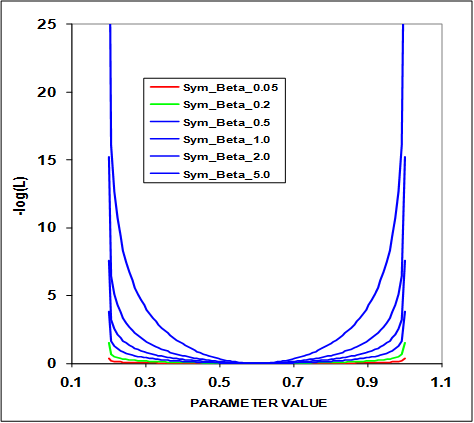
\includegraphics{Beta}\\
			Prior distributions for the symmetric beta distribution.
	\end{center}

\item \textbf{Prior Type = 2 = Beta prior}  \\ 
The definition of $\mu$ is consistent with CASAL's formulation with the $Bprior$ and $Aprior$ corresponding to the $m$ and $n$ parameters.
	\begin{equation}
		\mu = \frac{Prior-P_{min}}{P_{max}-P_{min}} 
        \end{equation}
	\begin{equation}
		\tau  = \frac{(Prior-P_{min})(P_{max}-Prior)}{Pr\_SD^2}-1
        \end{equation}
	\begin{equation}
		Bprior  = \tau \cdot \mu
        \end{equation}
	\begin{equation}
                Aprior = \tau (1-\mu)
        \end{equation}

	\begin{equation}
          \begin{split}
		\text{Prior Likelihood} = & (1 - Bprior) \cdot log(0.0001 + p - P_{min}) \\
		& + (1 - Aprior) \cdot log(0.0001 + P_{max} - p) \\
		& - (1 - Bprior) \cdot log(0.0001 + Prior - P_{min}) \\
		& - (1 - Aprior) \cdot log(0.0001 + P_{max} - Prior)
	  \end{split}
	\end{equation}

	\begin{center}
		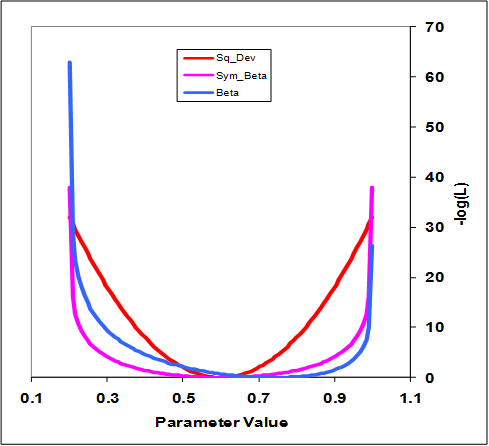
\includegraphics{BetaComparison}\\
		Comparison of the symmetric beta and the beta prior functions
	\end{center}

\item \textbf{Prior Type 3 = Lognormal prior} \\ 
Note that this is undefined for $p <= 0$ so the lower bound on the parameter must be > 0. The prior value is input into the parameter line in log space while the initial parameter value is defined in normal space (e.g. INIT = 0.20, PRIOR = -1.609438).
	\begin{equation}
	\text{Prior Likelihood} = \frac{1}{2} \left(\frac{log(p)-Prior}{Pr\_SD}\right)^2
	\end{equation}

\item \textbf{Prior Type 4 = Lognormal prior with bias correction} \\ 
This option is thanks to Larry Jacobson. Note that this is undefined for $p <= 0$ so the lower bound on the parameter must be > 0.
	\begin{equation}
	\text{Prior Likelihood} = \frac{1}{2} \left(\frac{log(p)-Prior + \frac{1}{2}{Pr\_SD}^2}{Pr\_SD}\right)^2
	\end{equation}

\item \textbf{Prior Type 5 = Gamma prior} \\ 
This option is thanks to Larry Jacobson. The lower bound should be 0 or greater.
	\begin{equation}
          scale = \frac{{Pr\_SD}^2}{Prior}
	\end{equation}
	\begin{equation}
          shape = \frac{Prior}{scale}
	\end{equation}
	\begin{equation}
          \text{Prior Likelihood} = -shape \cdot log(scale) - log\big(\Gamma(shape)\big) + (shape - 1) \cdot log(p) - \frac{p}{scale}
	\end{equation}

\item \textbf{Prior Type 6 = Normal prior} \\ 
Note that this function is independent of the parameter bounds.
		\begin{equation}
		\text{Prior Likelihood} = \frac{1}{2} \left(\frac{p - Prior}{Pr\_SD}\right)^2
		\end{equation}
\end{itemize}
